\documentclass[aspectratio=169]{beamer}
\usepackage{animate}
\usepackage{tikz}
\usetheme{metropolis}

% Bibliography setup
\usepackage{natbib}
\bibliographystyle{apalike}

\title{A Differentiable Bayesian Anomaly Detection Framework for Robust SALT3 Parameter Estimation Using \texttt{JAX}}
\subtitle{Sam Leeney}
\date{July 1, 2025}
\author{With: Will Handley, Harry Bevins, Eloy de Lera Acedo}
\institute{Nuclear Multimessenger Astronomy Group, Rotterdam}
\setbeamertemplate{footline}{
\leavevmode%
\hbox{%
\begin{beamercolorbox}[wd=.33\paperwidth,ht=2.5ex,dp=1ex,leftskip=3mm]{author in head/foot}%
\tiny Sam Leeney
\end{beamercolorbox}%
\begin{beamercolorbox}[wd=.33\paperwidth,ht=2.5ex,dp=1ex,center]{title in head/foot}%
\tiny sakl2@cam.ac.uk
\end{beamercolorbox}%
\begin{beamercolorbox}[wd=.33\paperwidth,ht=2.5ex,dp=1ex,rightskip=3mm]{date in head/foot}%
\tiny \href{https://github.com/samleeney}{github.com/samleeney/Talks}
\end{beamercolorbox}%
}%
\vskip0pt%
}


\begin{document}

\begin{frame}
  \begin{center}
    % Title
    {\Large A Differentiable Bayesian Anomaly Detection Framework for Robust SALT3 Parameter Estimation Using \texttt{JAX-bandflux}\par}
    \vspace{0.3cm}

    % Subtitle
    {\normalsize Sam Leeney\par}
    \vspace{0.3cm}

    % Conference and Date
    {\small Nuclear Multimessenger Astronomy Group\par}
    {\small July 1, 2025\par}
    \vspace{0.5cm}

    % Co-authors
    {\scriptsize With: Will Handley, Harry Bevins, Eloy de Lera Acedo\par}
    \vfill

    % Affiliations image at the bottom
    
\includegraphics[width=0.9\textwidth]{images/affiliations.png}
  \end{center}
\end{frame}

\begin{frame}{Outline}
  \tableofcontents[hideallsubsections]
\end{frame}


\section{Bayesian anomaly detection}

\begin{frame}{Over simplified example of anomaly detection method (thresholding)}
  \begin{columns}
    \column{0.5\textwidth}
    \textbf{Constant signal with anomalies:}
    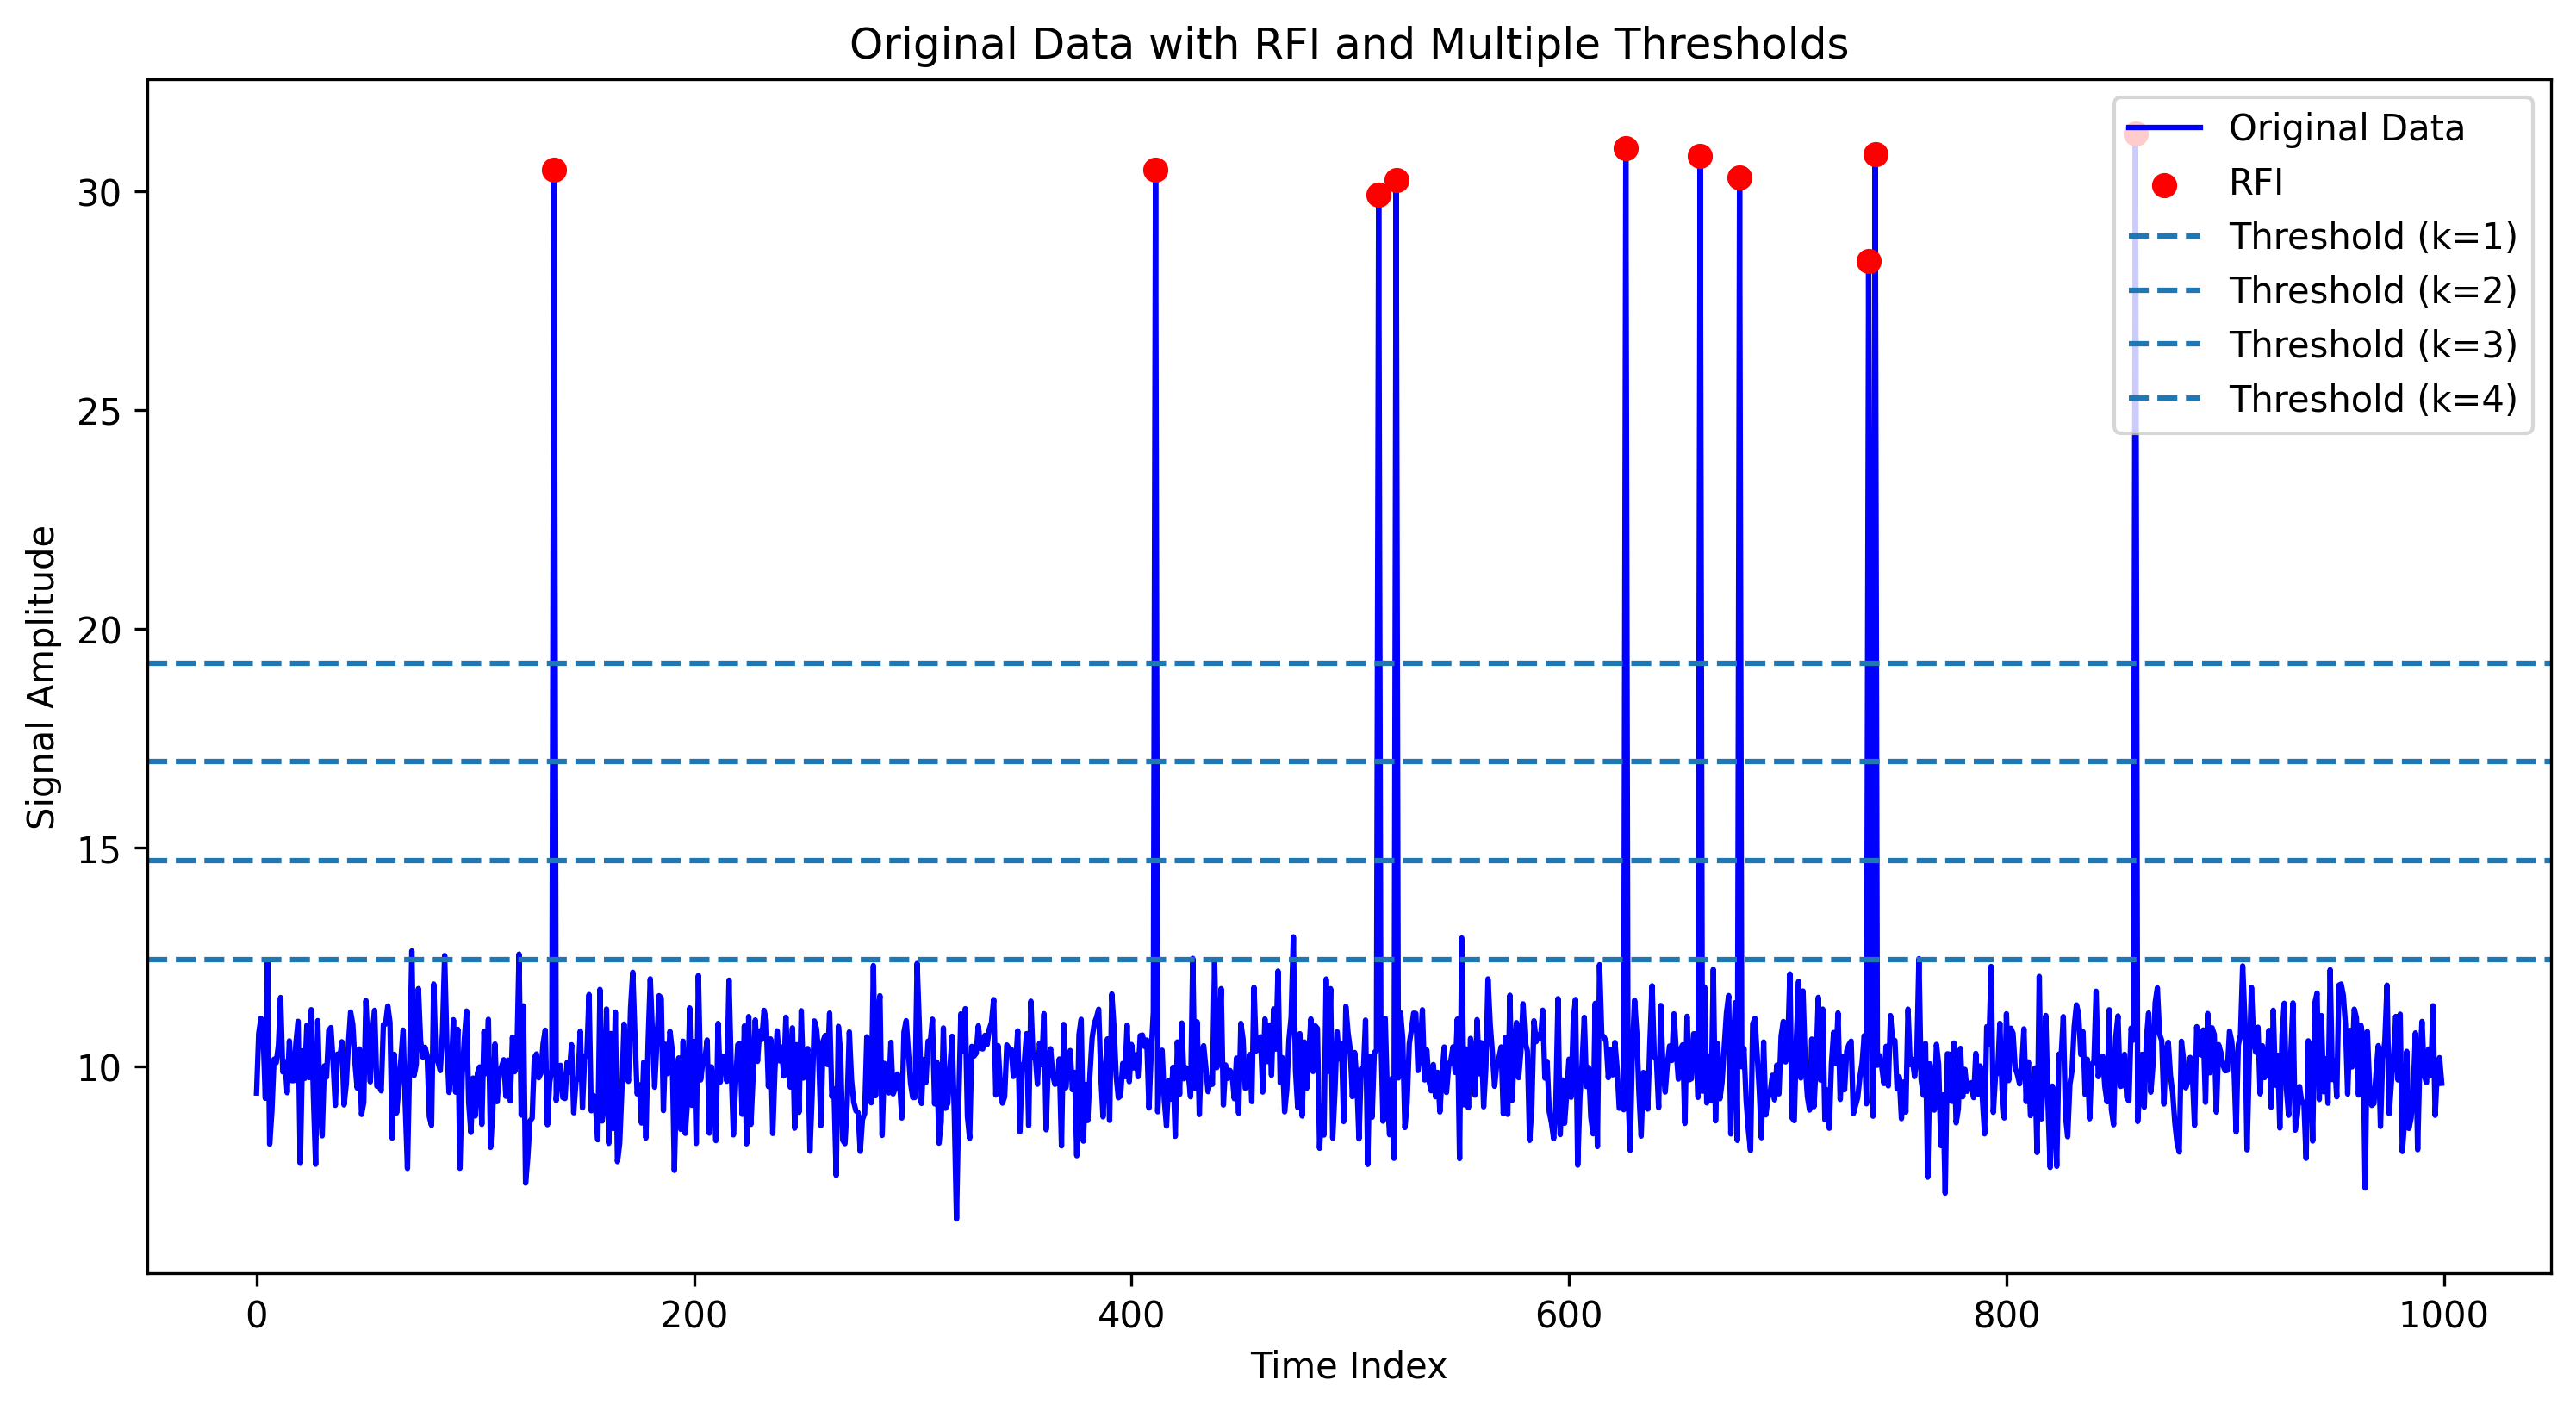
\includegraphics[width=1\textwidth]{images/threshold_multiple.png}
    \column{0.5\textwidth}
    \textbf{Sine wave with anomalies:}
    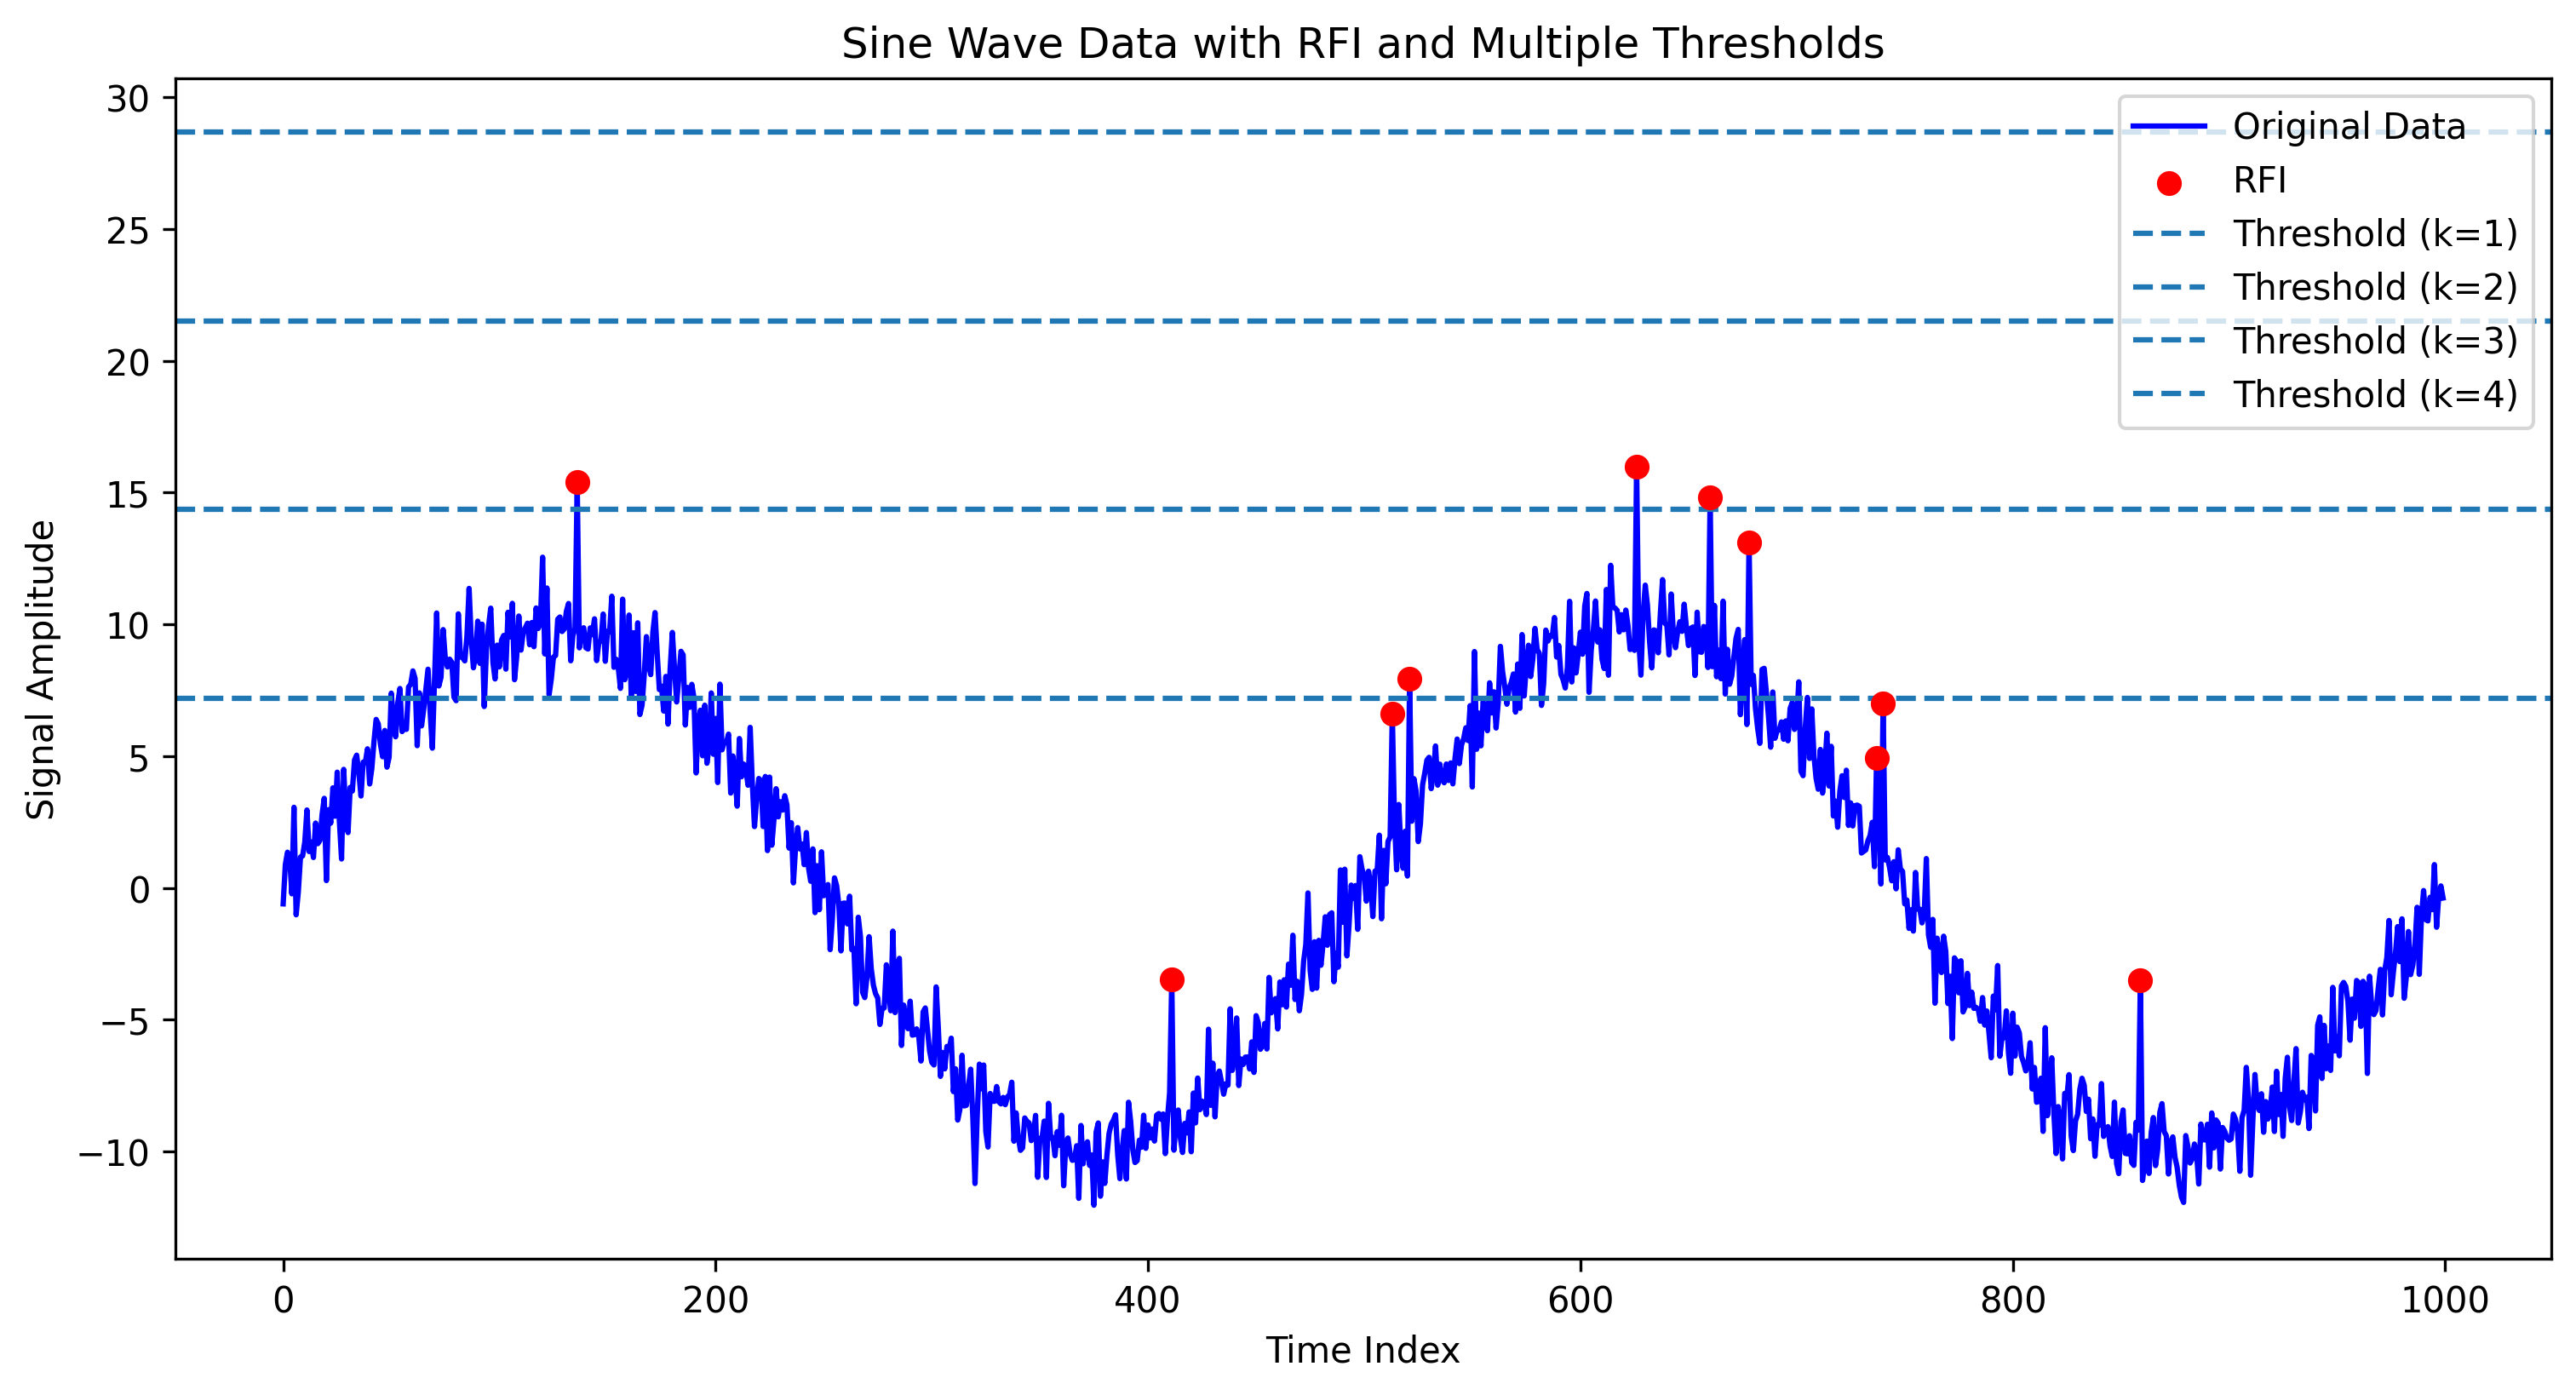
\includegraphics[width=1\textwidth]{images/threshold_sin_multiple.png}
  \end{columns}
  \begin{itemize}
    \item Traditional methods are generally not model aware.
    \item Anomalies are typically sought either before or after typical fitting process.
  \end{itemize}
\end{frame}

\begin{frame}{Model anomalies in via a method that is:}
  We want a method that is...
  \begin{itemize}
    \item Model aware
    \item Works simultaneously with model fitting
    \item Not binary, ie encodes 'belief' datum are anomalous
  \end{itemize}
\end{frame}

\begin{frame}{Bayes' Theorem}
  \begin{columns}
    \column{0.6\textwidth}
    \textbf{Bayes' Theorem:}
    \begin{equation}
        P(\theta | \mathcal{D}) = \frac{P(\mathcal{D} | \theta) P(\theta)}{P(\mathcal{D})}
    \end{equation}
    Where:
    \begin{itemize}
        \item $P(\theta | \mathcal{D})$: Posterior (updated belief)
        \item $P(\mathcal{D} | \theta)$: Likelihood (model prediction)
        \item $P(\theta)$: Prior (initial belief)
        \item $P(\mathcal{D})$: Evidence (model comparison)
    \end{itemize}
    
    \column{0.4\textwidth}
    \begin{center}
    \textbf{The Challenge:}
    \vspace{0.5cm}
    
    \textit{We need some way of incorporating anomalous data points natively into our likelihood.}
    \vspace{0.5cm}
    
    Standard likelihoods cannot account for this.
    \end{center}
  \end{columns}
\end{frame}

\begin{frame}{Define anomaly mask $\varepsilon$}
  \begin{columns}
    \column{0.25\textwidth} % Equation on the left, 25% width
      \footnotesize
      \begin{equation}
          \varepsilon_i = \begin{cases}
              0 &: \text{expected}\\
              1 &: \text{anomalous},
          \end{cases}
      \end{equation}
    \column{0.75\textwidth} % Image on the right, 75% width
      \centering
      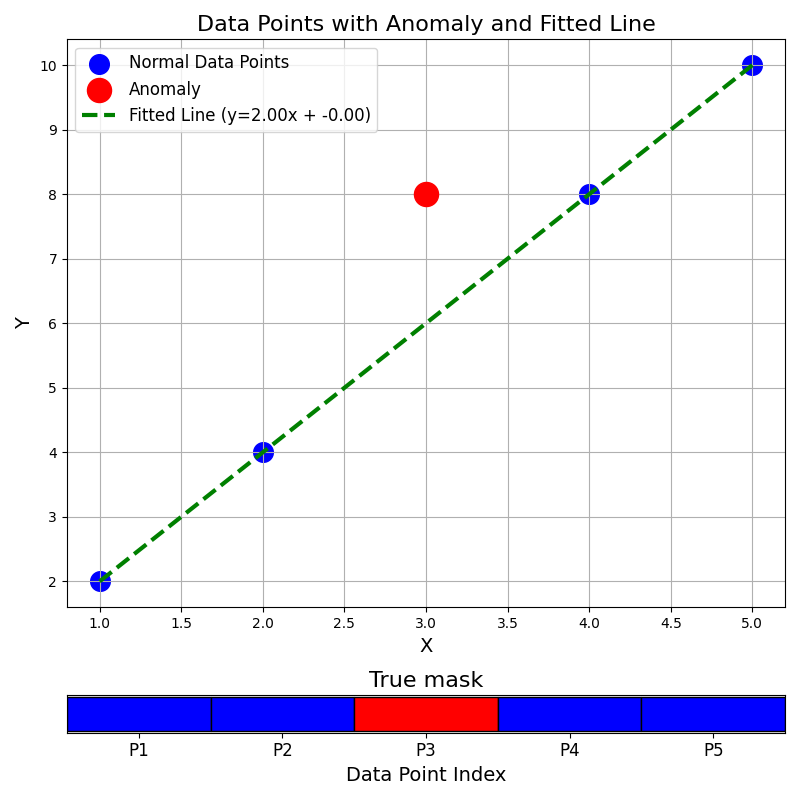
\includegraphics[width=0.7\textwidth]{images/generated_plot.png} % Image should fill its column
  \end{columns}
\end{frame}

\begin{frame}{Ascribe Bernoulli prior to $\varepsilon$}
  \footnotesize
  \begin{equation}
      P(\varepsilon_i) = p^{\varepsilon_i}(1-p)^{(1-\varepsilon_i)}.
  \end{equation}
  \begin{itemize}
    \item A Bernoulli prior assigns a probability $p$ to a binary variable being 1 (anomalous) and $1-p$ to it being 0 (expected).
  \end{itemize}
\end{frame}


\begin{frame}{Piecewise likelihood with $\varepsilon$}
    \centering
    The likelihood function before marginalizing over $\epsilon$ is given by:
    $$P(\vec{D}, \vec{\epsilon} | \theta) = \prod_{i=1}^{N} \left(L_i(\theta) (1-p)\right)^{(1-\epsilon_i)} \left(\frac{p}{\Delta}\right)^{\epsilon_i}$$
    Where:
    \begin{itemize}
        \item $L_i(\theta)$ is the likelihood of the $i$'th data point $D_i$ under the "expected" model.
        \item $\Delta$ is a constant related to the "anomalous" model.
        \item $p$ is the prior probability that a data point is anomalous ($P(\epsilon_i = 1)$).
        \item $\epsilon_i$ is a binary variable: $\epsilon_i = 0$ for expected, $\epsilon_i = 1$ for anomalous.
    \end{itemize}
\end{frame}

\begin{frame}{Marginalise over epsilon}
  \footnotesize
  \begin{equation}
      P(\mathcal{D} | \theta) =\sum_{\varepsilon \in \{ 0, 1 \} ^N}P(\mathcal{D},\varepsilon|\theta)
  \end{equation}
  \begin{center}
    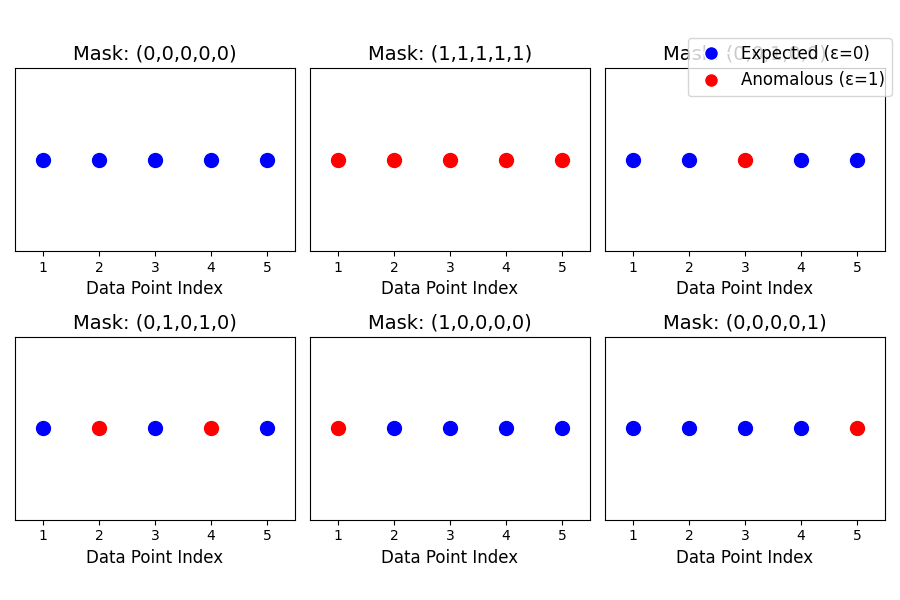
\includegraphics[width=0.64\textwidth]{images/marginalize_epsilon_plot.png}
  \end{center}
\end{frame}
\begin{frame}{Likelihood After Marginalization}
    \centering
    The likelihood function after marginalizing over $\epsilon$ is given by:
    $$L(D | \theta) = \prod_{i=1}^{N} \left( (1-p) L_i(\theta) + p \frac{1}{\Delta} \right)$$
    Where:
    \begin{itemize}
        \item $D = \{D_1, D_2, \dots, D_N\}$ represents the dataset of $N$ data points.
        \item $\theta$ represents the model parameters.
        \item $L_i(\theta)$ is the likelihood of the $i$-th data point $D_i$ being "expected".
        \item $p$ is the prior probability that a single data point is "anomalous".
        \item This is computationally impractical as mask scales $2^N$.
    \end{itemize}
\end{frame}

\begin{frame}{Approximate correct mask is most likely}
  \footnotesize
  \begin{equation}
      P(\mathcal{D}|\theta, \varepsilon_{\mathrm{max}}) \gg \mathrm{max}_j P(\mathcal{D}|\theta,\varepsilon^{(j)})\label{eq:nlo},
  \end{equation}
  \begin{center}
    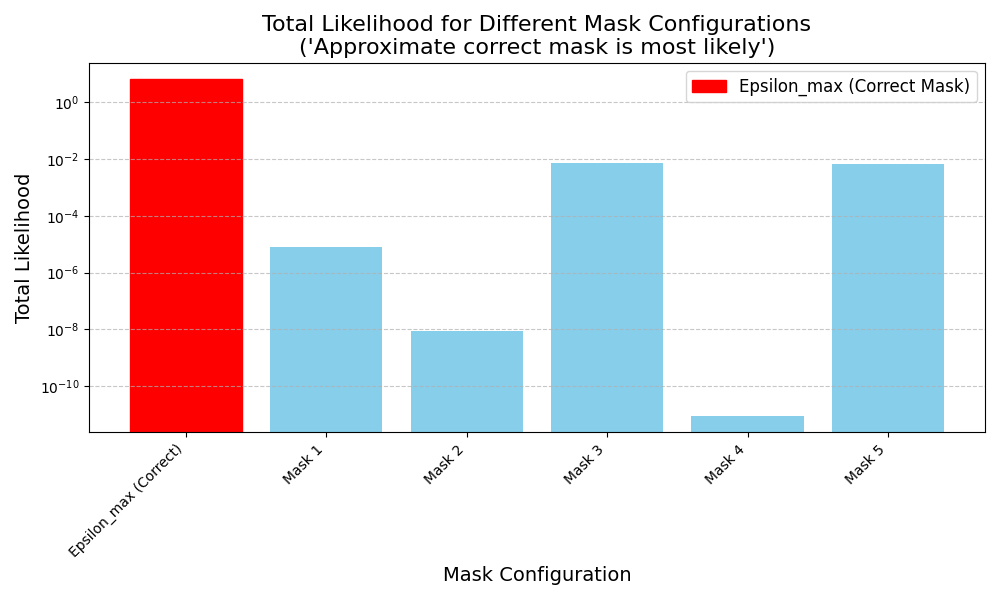
\includegraphics[width=0.64\textwidth]{images/dominant_mask_plot.png}
  \end{center}
\end{frame}

\begin{frame}{Loglikelihood and Maximisation}
  \footnotesize
  \textbf{e) Loglikelihood:}
  \begin{align}
      \log{P(\mathcal{D}|\theta)} &= \sum_{i}[\log{\mathcal{L}_i}+\log(1-p)]\varepsilon^{\mathrm{max}}_i \nonumber\\
      &\quad + [\log{p} - \log{\Delta}](1 - \varepsilon^\mathrm{max}_i)
  \end{align}

  \textbf{f) Find the mask $\varepsilon^{max}$ that maximises the likelihood:}
  \begin{equation}
  \log P(\mathcal{D}|\theta) =
  \begin{cases}
  \log \mathcal{L}_i + \log(1 - p), & \text{if } \log \mathcal{L}_i + \log(1 - p) > \log p - \log \Delta \\
  \log p - \log \Delta, & \text{otherwise}
  \end{cases}
  \end{equation}
\end{frame}

\begin{frame}{We are imposing a 'floor' on our likelihood}
    \begin{columns}
        \column{0.5\textwidth}
            \centering
            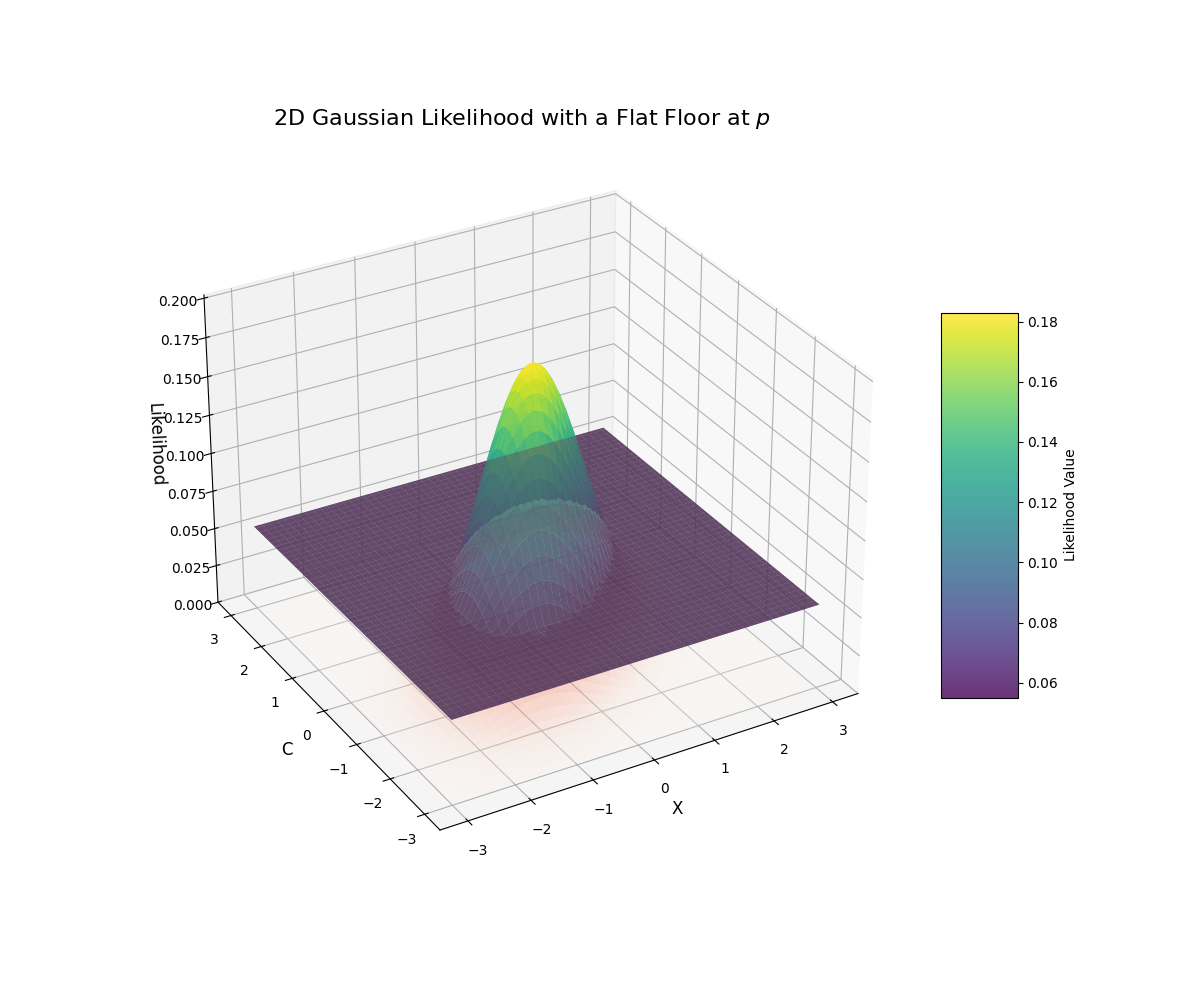
\includegraphics[width=1.2\textwidth]{images/likelihood_floor_plot.png}
        \column{0.5\textwidth}
            \centering
            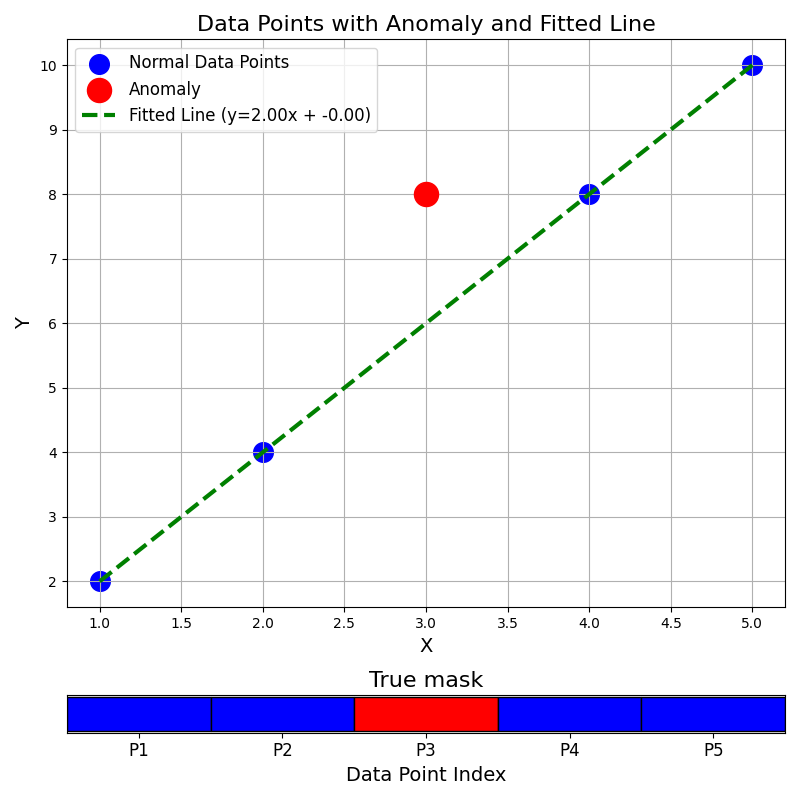
\includegraphics[width=0.7\textwidth]{images/generated_plot.png}
    \end{columns}
\end{frame}

\begin{frame}{Connection to the Logit Function}
  \footnotesize
  The condition for selecting between expected and anomalous data:
  \begin{equation}
    \log \mathcal{L}_i + \log(1-p) > \log p - \log \Delta
  \end{equation}
  
  Rearranging:
  \begin{equation}
    \log \mathcal{L}_i + \log \Delta > \log p - \log(1-p) = \log\left(\frac{p}{1-p}\right)
  \end{equation}
  
  The right-hand side is the \textbf{logit function}:
  \begin{equation}
    \text{logit}(p) = \log\left(\frac{p}{1-p}\right)
  \end{equation}
  
  \begin{itemize}
    \item Logit is the inverse of the sigmoid function
    \item Maps probability $p \in (0,1)$ to $(-\infty, +\infty)$
    \item Common activation function in machine learning for binary classification
    \item Naturally encodes our degree of belief in each datum's integrity
  \end{itemize}
\end{frame}

\begin{frame}{Derivation Summary}
  \footnotesize
  \textbf{1. Define anomaly mask:} $\varepsilon_i \in \{0, 1\}$ for each data point
  
  \textbf{2. Bernoulli prior:} $P(\varepsilon_i) = p^{\varepsilon_i}(1-p)^{(1-\varepsilon_i)}$
  
  \textbf{3. Piecewise likelihood:} $P(\vec{D}, \vec{\epsilon} | \theta) = \prod_{i=1}^{N} \left(L_i(\theta) (1-p)\right)^{(1-\epsilon_i)} \left(\frac{p}{\Delta}\right)^{\epsilon_i}$
  
  \textbf{4. Marginalize over $\epsilon$:} $P(\mathcal{D} | \theta) = \sum_{\varepsilon \in \{ 0, 1 \} ^N}P(\mathcal{D},\varepsilon|\theta)$
  
  \textbf{5. Dominant mask approximation:} $P(\mathcal{D}|\theta, \varepsilon_{\mathrm{max}}) \gg \mathrm{max}_j P(\mathcal{D}|\theta,\varepsilon^{(j)})$
  
  \textbf{6. Final loglikelihood}
  \begin{equation*}
  \log P(\mathcal{D}|\theta) =
  \begin{cases}
  \log \mathcal{L}_i + \log(1 - p), & \text{if } \log \mathcal{L}_i + \log(1 - p) > \log p - \log \Delta \\
  \log p - \log \Delta, & \text{otherwise}
  \end{cases}
  \end{equation*}
  
  \vfill
  \centering
  \textbf{Any questions on the derivation before we proceed?}
\end{frame}

\begin{frame}{Fit on a simple toy model}
  \begin{columns}
    \column{0.7\textwidth}
    \centering
    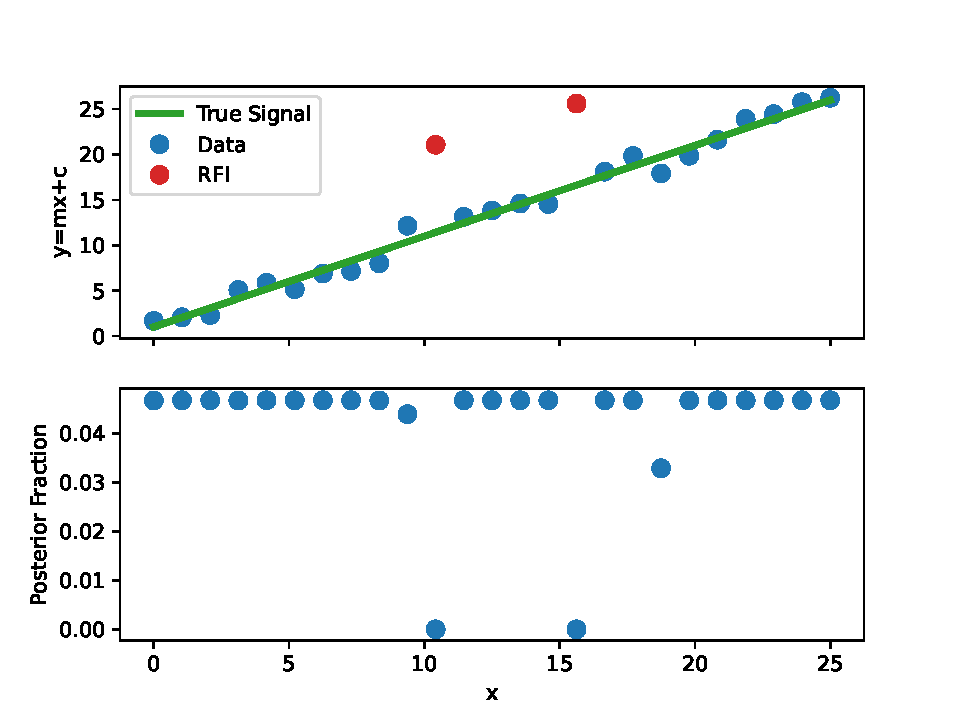
\includegraphics[width=0.8\textwidth]{images/test.pdf}
    \column{0.3\textwidth}
    \footnotesize
    \textbf{Posterior fraction:}
    \begin{equation}
        f_i = P(\varepsilon_i = 1 | \mathcal{D}, \theta)
    \end{equation}
    Posterior probability that data point $i$ is anomalous. Non-contaminated points have $f_i \approx 0.04$ (baseline level for 25 data points).
  \end{columns}
\end{frame}

\begin{frame}{Varying $p$}
    \centering
    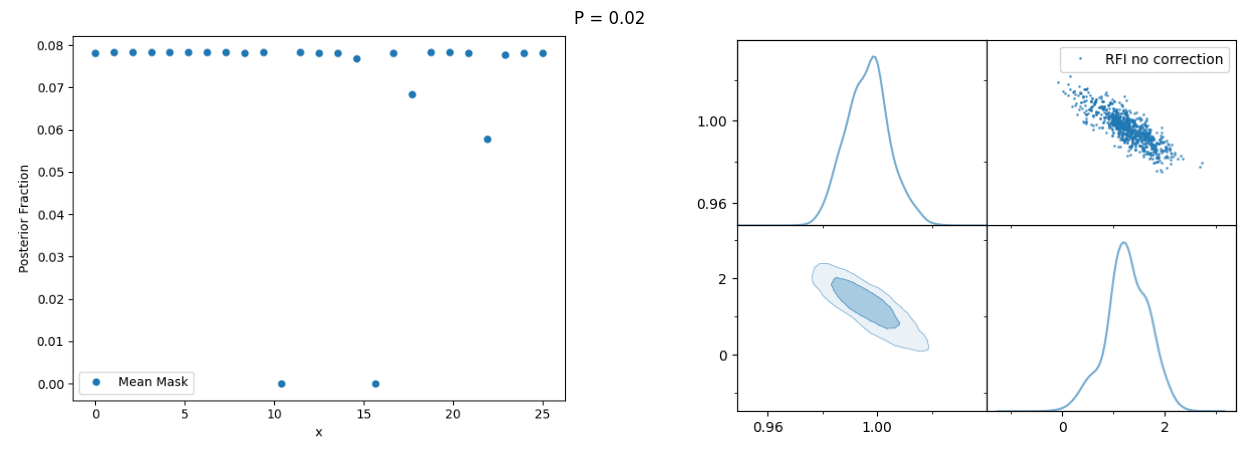
\includegraphics[width=0.8\textwidth]{images/gif_anest/comb_2.png}
\end{frame}

\begin{frame}{Varying $p$}
    \centering
    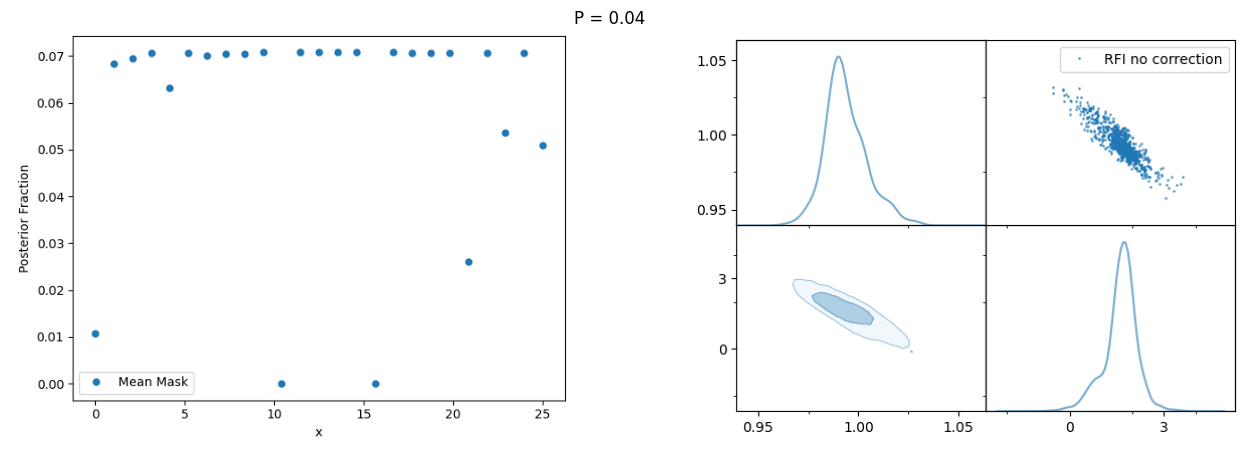
\includegraphics[width=0.8\textwidth]{images/gif_anest/comb_3.png}
\end{frame}


\begin{frame}{Varying $p$}
    \centering
    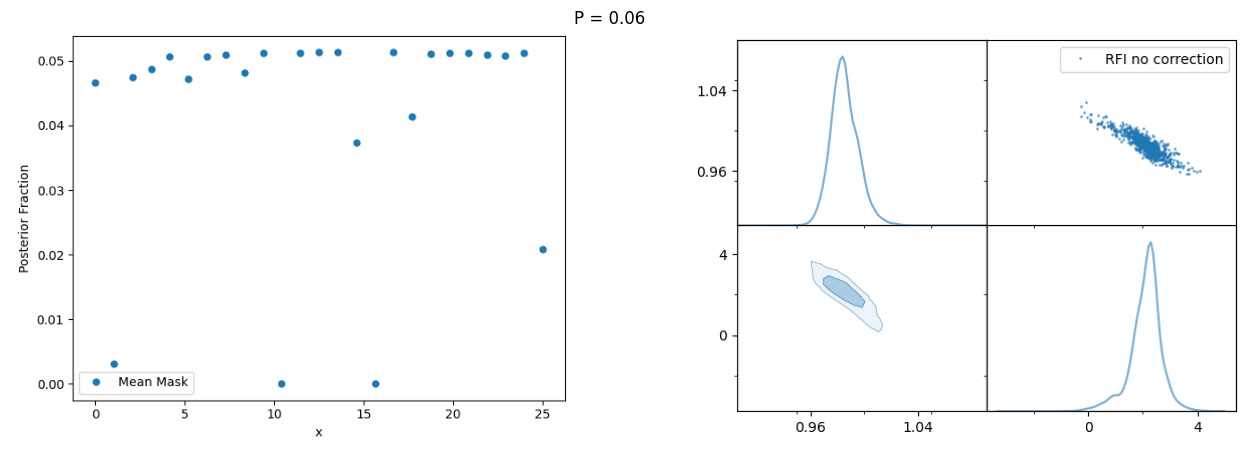
\includegraphics[width=0.8\textwidth]{images/gif_anest/comb_4.png}
\end{frame}

\begin{frame}{Varying $p$}
    \centering
    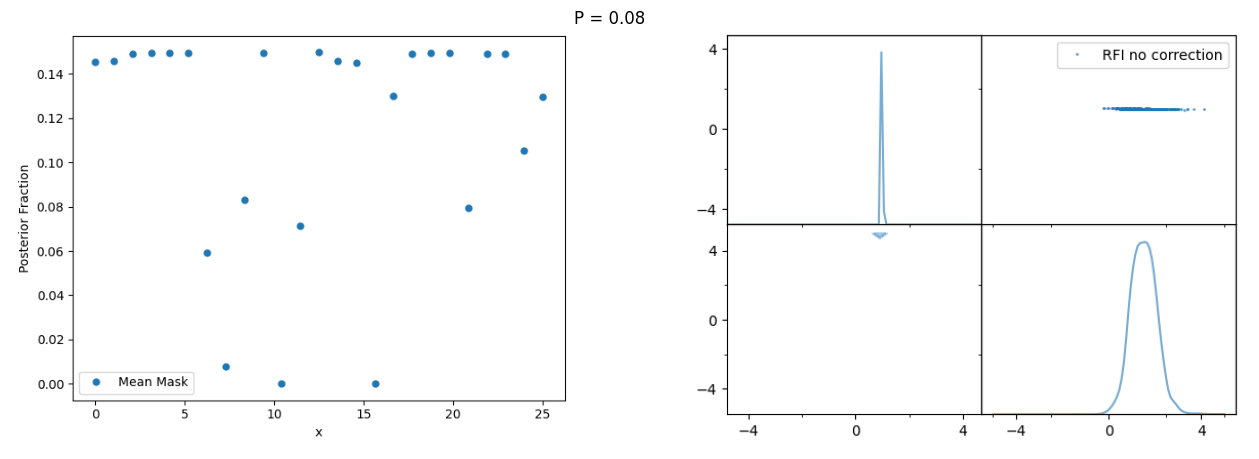
\includegraphics[width=0.8\textwidth]{images/gif_anest/comb_5.png}
\end{frame}

\begin{frame}{Varying $p$}
    \centering
    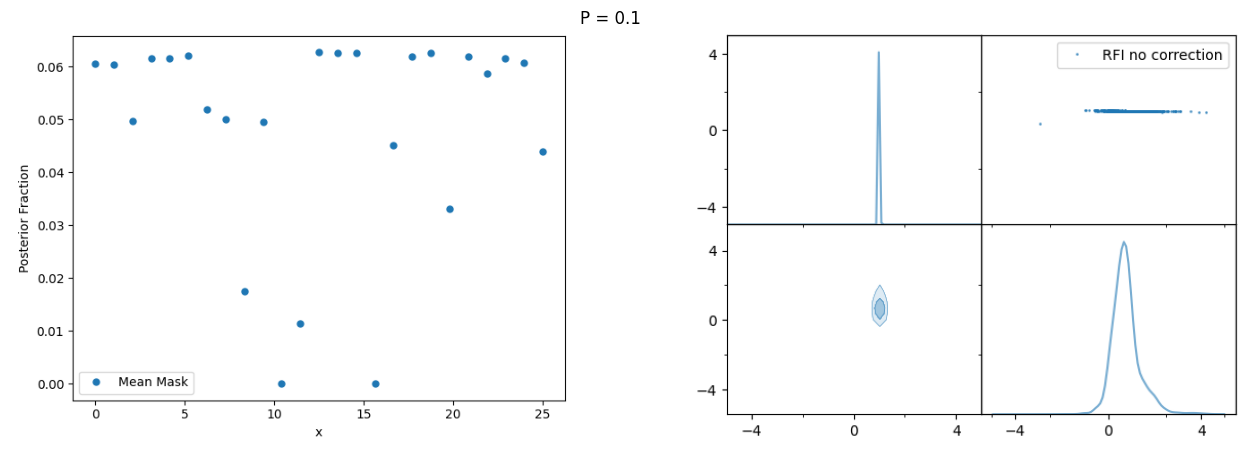
\includegraphics[width=0.8\textwidth]{images/gif_anest/comb_6.png}
\end{frame}

\begin{frame}{Varying $p$}
    \centering
    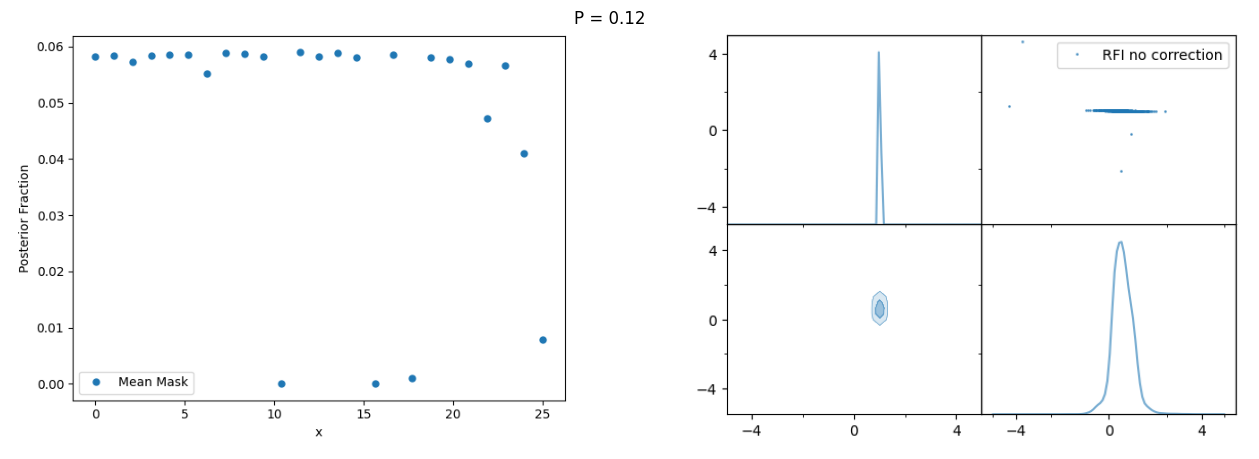
\includegraphics[width=0.8\textwidth]{images/gif_anest/comb_7.png}
\end{frame}

\begin{frame}{Varying $p$}
    \centering
    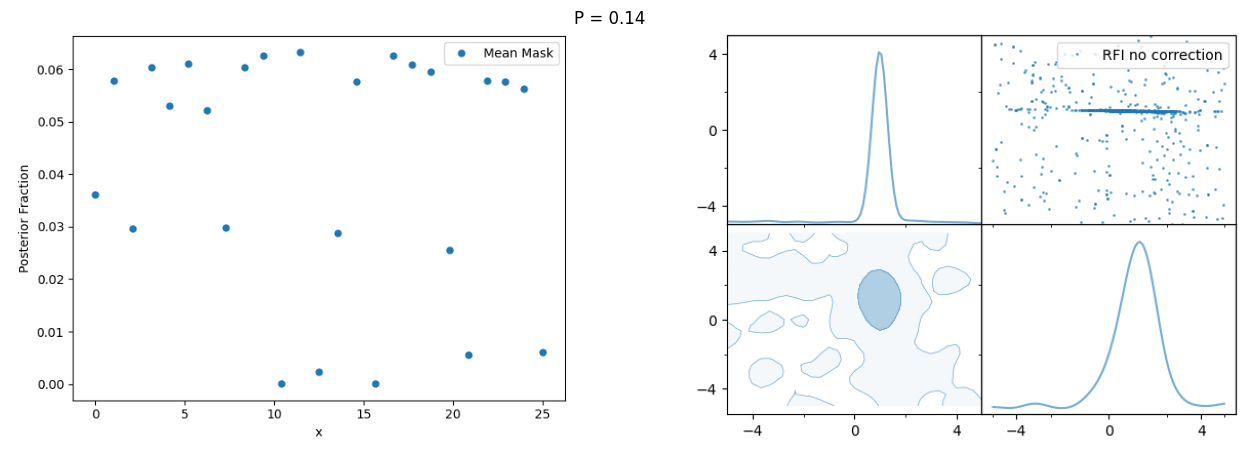
\includegraphics[width=0.8\textwidth]{images/gif_anest/comb_8.png}
\end{frame}

\begin{frame}{Varying $p$}
    \centering
    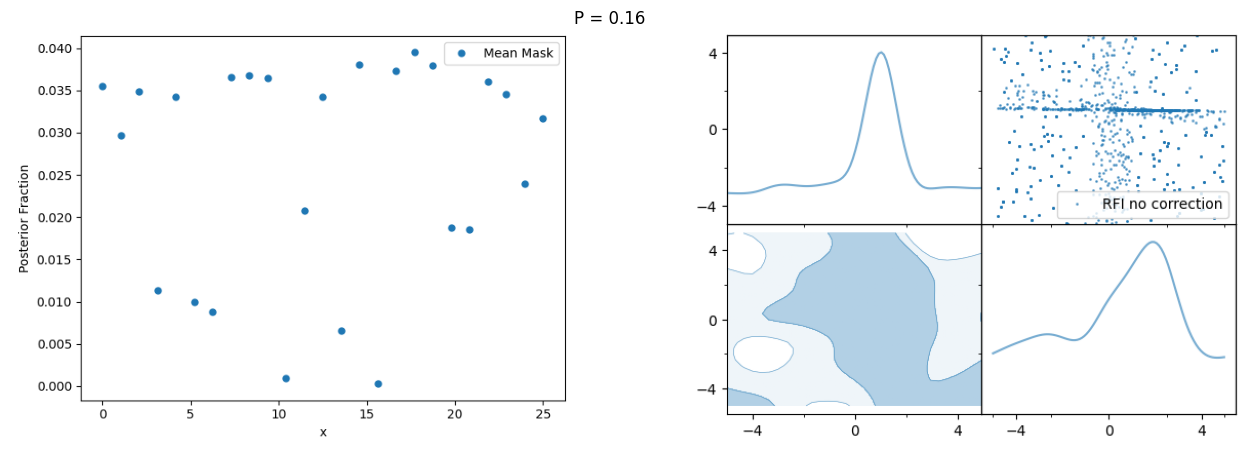
\includegraphics[width=0.8\textwidth]{images/gif_anest/comb_9.png}
\end{frame}


\begin{frame}{Selection strategy for $p$.}
  \begin{columns}
    \column{0.5\textwidth}
    \begin{itemize}
      \item `Select $p$ such that the Bayesian evidence is maximised'
    \end{itemize}
    \column{0.5\textwidth}
    \begin{figure}
      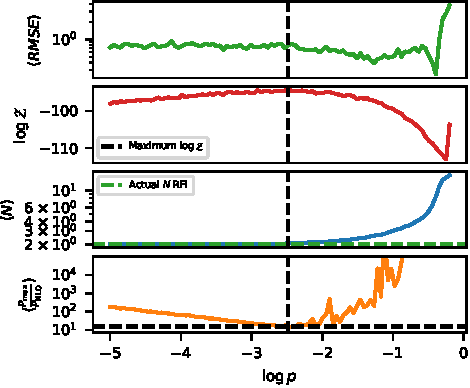
\includegraphics[width=0.8\textwidth]{images/f_approx_current_sig5_2.pdf}
    \end{figure}
  \end{columns}
\end{frame}

\begin{frame}{Fully automated anomaly detection}
  \begin{itemize}
  \item Putting a prior on $p$, we can fit it dynamically as a free parameter.
  \item This fully automates the anomaly detection process.
  \item Must exclude $p=0$.
  \end{itemize}
\end{frame}

\begin{frame}{Application to toy model}
  \centering
  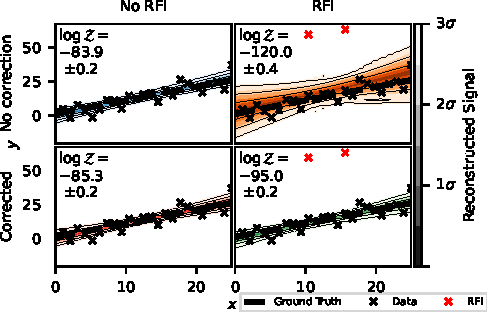
\includegraphics[width=0.64\textwidth]{images/4pane_toy_sidebar.pdf}
\end{frame}

\begin{frame}{Implement with 2 lines of code}
  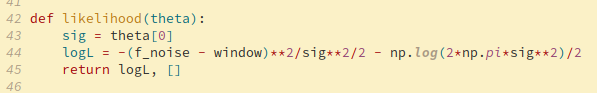
\includegraphics[width=1\textwidth]{images/logl1.png}
  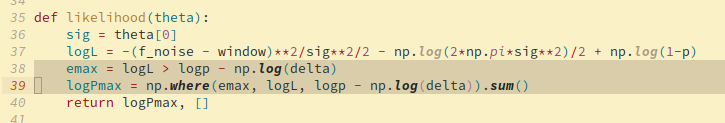
\includegraphics[width=1\textwidth]{images/logl2.png}
  \centering Tutorial @ github.com/samleeney
\end{frame}

\begin{frame}{Read the paper!}
  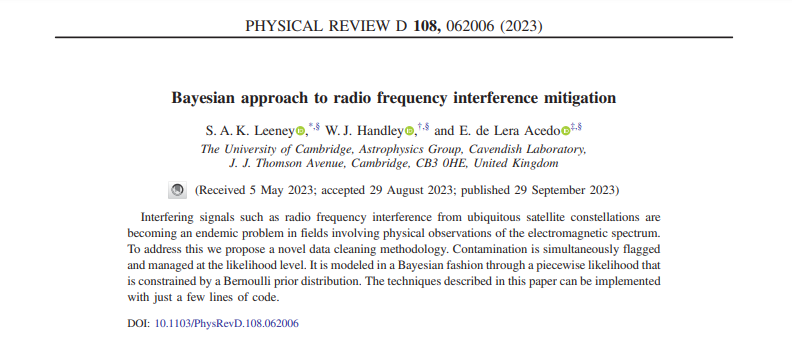
\includegraphics[width=1\textwidth]{images/paper1.png}
  \href{https://arxiv.org/abs/2211.15448}{arxiv: 2211.15448}
\end{frame}


\section{Bayesian anomaly detection for Ia Supernovae}

\begin{frame}{Supernovae Cosmology: Two Key Requirements}
  \begin{itemize}
    \item \textbf{Standardisation Method:} Need a way to standardise and compare other supernovae
      \begin{itemize}
        \item Corrects for intrinsic variations between SNe
        \item Makes them useful as standard candles
      \end{itemize}
    \item \textbf{Distance Anchor:} Need absolute distance calibration for some supernovae
      \begin{itemize}
        \item Provides the absolute magnitude scale
        \item Converts apparent magnitudes to distances
      \end{itemize}
  \end{itemize}
  \vfill
  \centering
  \textbf{Both components are essential for cosmological measurements}
\end{frame}

\begin{frame}{Distance Anchor Methods}
  \begin{columns}
    \column{0.5\textwidth}
    \textbf{Distance Ladder:}
    
    Builds up from nearby geometric distances to farther objects using overlapping standard candles. Each rung calibrates the next, propagating uncertainties upward.
    
    \column{0.5\textwidth}
    \textbf{Assumes Some Cosmology:}
    
    Uses early universe physics and standard cosmological model to predict distances. Independent of local measurements but requires assumptions about dark energy and matter.
  \end{columns}
  \vfill
  \centering
  \textbf{H$_0$ tension: These methods give different results!}
\end{frame}

\begin{frame}{Standardising Supernovae}
  \begin{center}
  \fbox{
    \begin{minipage}{0.9\linewidth}
      \centering
      \footnotesize
      \textbf{Key idea:} If we can anchor one supernova's distance, we can standardise and compare it to all others
    \end{minipage}
  }
  \end{center}
  \vfill
  \begin{columns}
    \column{0.4\textwidth}
    \scriptsize
    \textbf{The Problem:}
    \begin{itemize}
      \item SNe with higher stretch fade more slowly
      \item Redder SNe appear dimmer (dust)
      \item Prevents direct distance comparisons
    \end{itemize}
    \vspace{0.3cm}
    \textbf{The Solution:}
    \begin{itemize}
      \item Measure stretch ($x_1$) and color ($c$)
      \item Apply SALT corrections
      \item Reveal common peak luminosity
    \end{itemize}
    \column{0.6\textwidth}
    \centering
    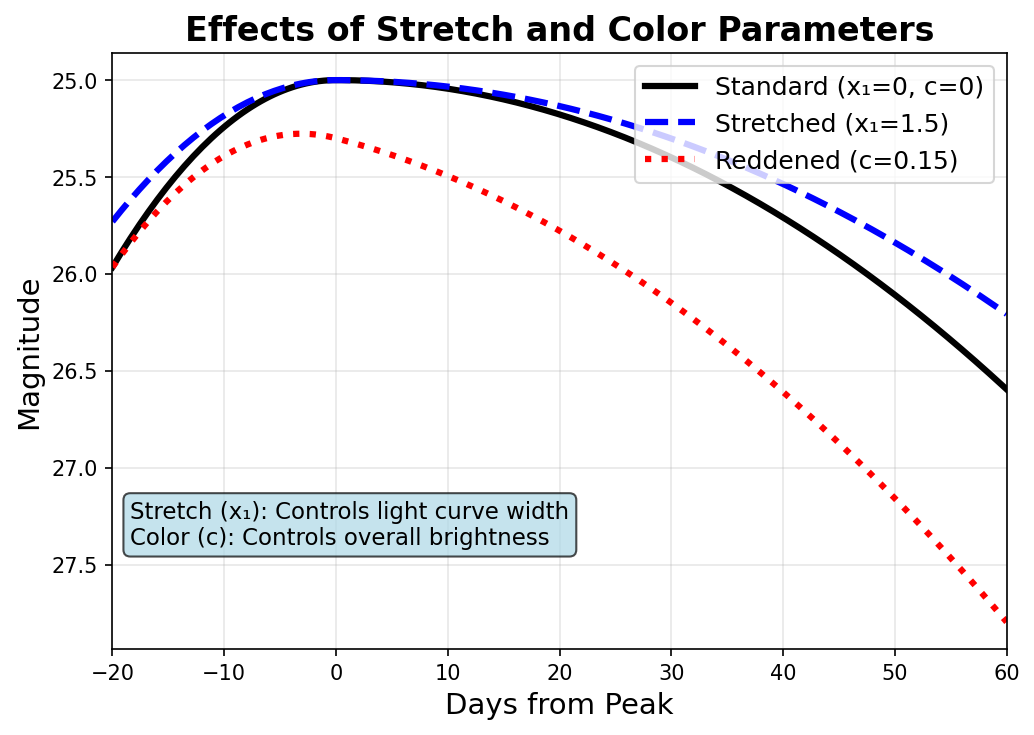
\includegraphics[width=0.9\textwidth]{images/stretch_color_effects_plot.png}
  \end{columns}
\end{frame}

\begin{frame}{Standardisation Methods}
  \begin{columns}
    \column{0.5\textwidth}
    \textbf{SALT Model (Spectral Adaptive Light curve Template):}
    \begin{itemize}
      \item State-of-the-art standardisation method
      \item Parameters:
        \begin{itemize}
          \item $x_0$: amplitude/brightness
          \item $x_1$: stretch factor
          \item $c$: color parameter
        \end{itemize}
      \item Tripp formula: $\mu = m_B - M_B + \alpha x_1 - \beta c$
    \end{itemize}
    
    \column{0.5\textwidth}
    \textbf{Other Methods:}
    \begin{itemize}
      \item SNooPy (Carnegie Supernova Project)
      \item MLCS2k2 (Multi-Color Light Curve Shape)
      \item SiFTO (SN Ia Fitter using Templates)
      \item BayeSN (Bayesian approach)
    \end{itemize}
    \vspace{0.5cm}
    \centering
    \fbox{
      \begin{minipage}{0.9\linewidth}
        \centering
        \textbf{All methods aim to reveal:}
        
        $M_B \approx -19.3$ at peak
      \end{minipage}
    }
  \end{columns}
\end{frame}

\begin{frame}{The SALT3 Model for Supernovae}
  \begin{columns}
    \column{0.6\textwidth}
      \small
      \begin{itemize}
        \item \textbf{The Inverse Problem:} We observe flux measurements $F_{\text{obs}}(\lambda, t)$ and want to estimate SALT parameters
        \item Given observations, infer:
          \begin{itemize}
            \item $x_0$: brightness scaling
            \item $x_1$: stretch (width)
            \item $c$: colour
          \end{itemize}
        \item Use SALT3 model as our forward model to relate parameters to observations
      \end{itemize}
    \column{0.4\textwidth}
      \centering
      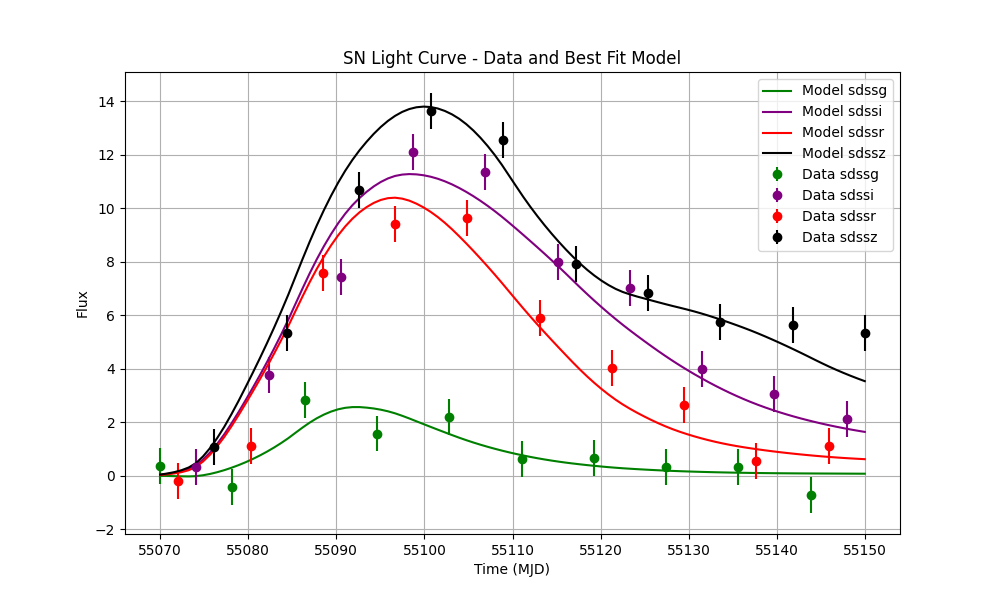
\includegraphics[width=0.9\textwidth]{images/sncosmo-fitter.png}
  \end{columns}
  \vfill
  \centering
  \footnotesize
  Forward model (SALT):
  \begin{equation*}
    F(p, \lambda) = x_0 \left[M_0(p, \lambda) + x_1M_1(p, \lambda) + \dots\right] \times \exp \left[c \times CL(\lambda)\right]
  \end{equation*}
  Bandflux:
  \begin{equation*}
    F_{\text{band}} = \int_{\lambda_{\text{min}}}^{\lambda_{\text{max}}} F(p, \lambda) \cdot T(\lambda) \cdot \frac{\lambda}{hc} d\lambda
  \end{equation*}
\end{frame}



\section{Fitting SALT models with \texttt{JAX-bandflux}}

\begin{frame}{\texttt{JAX-bandflux}}
  \begin{center}
    \begin{tikzpicture}
      % Draw oval
      \draw[thick] (0,0) ellipse (3.5cm and 2.5cm);
      
      % Place images in corners of oval
      \node at (-1.8, 1.2) {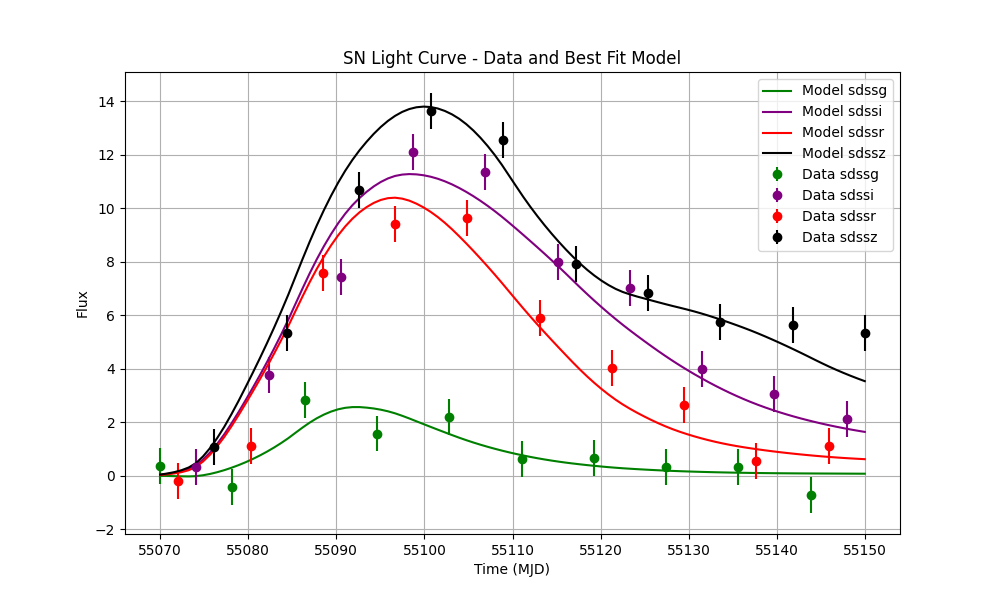
\includegraphics[width=3cm]{images/sncosmo-fitter.png}};
      \node at (1.8, 1.2) {
\includegraphics[width=3cm]{images/sncosmobanner.png}};
      \node at (-1.8, -1.2) {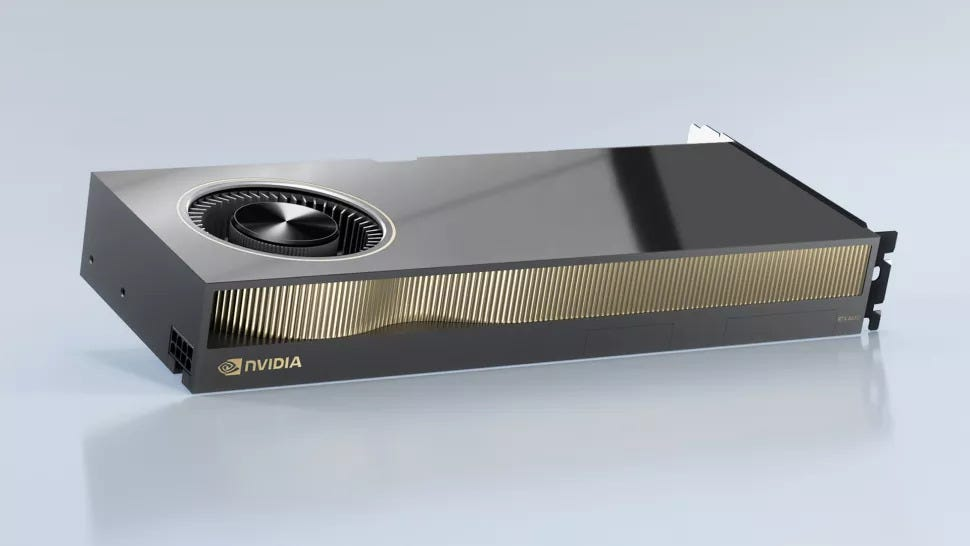
\includegraphics[width=3cm]{images/gpu.jpg}};
      \node at (1.8, -1.2) {
\includegraphics[width=3cm]{images/jax_logo_250px.png}};
    \end{tikzpicture}
  \end{center}
\end{frame}

\begin{frame}{\texttt{JAX-bandflux}: A Tool for Supernovae Analysis}
  \centering 
  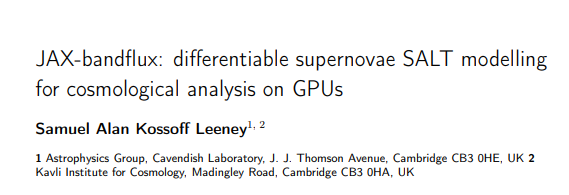
\includegraphics[width=0.8\textwidth]{images/josjaxbflux.png}
  \vspace{0.5cm}
  
  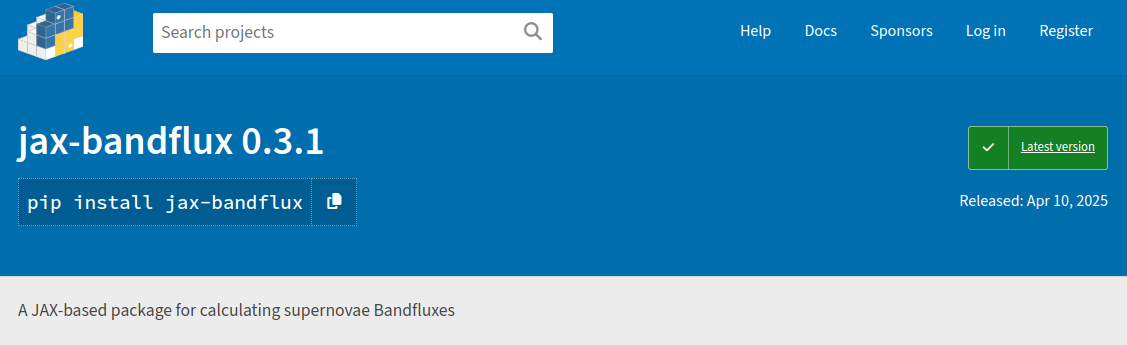
\includegraphics[width=0.6\textwidth]{images/pip-jax-bandflux.png}
\end{frame}

\begin{frame}{GPU vs CPU}
  \begin{columns}
    \column{0.5\textwidth}
      \centering
      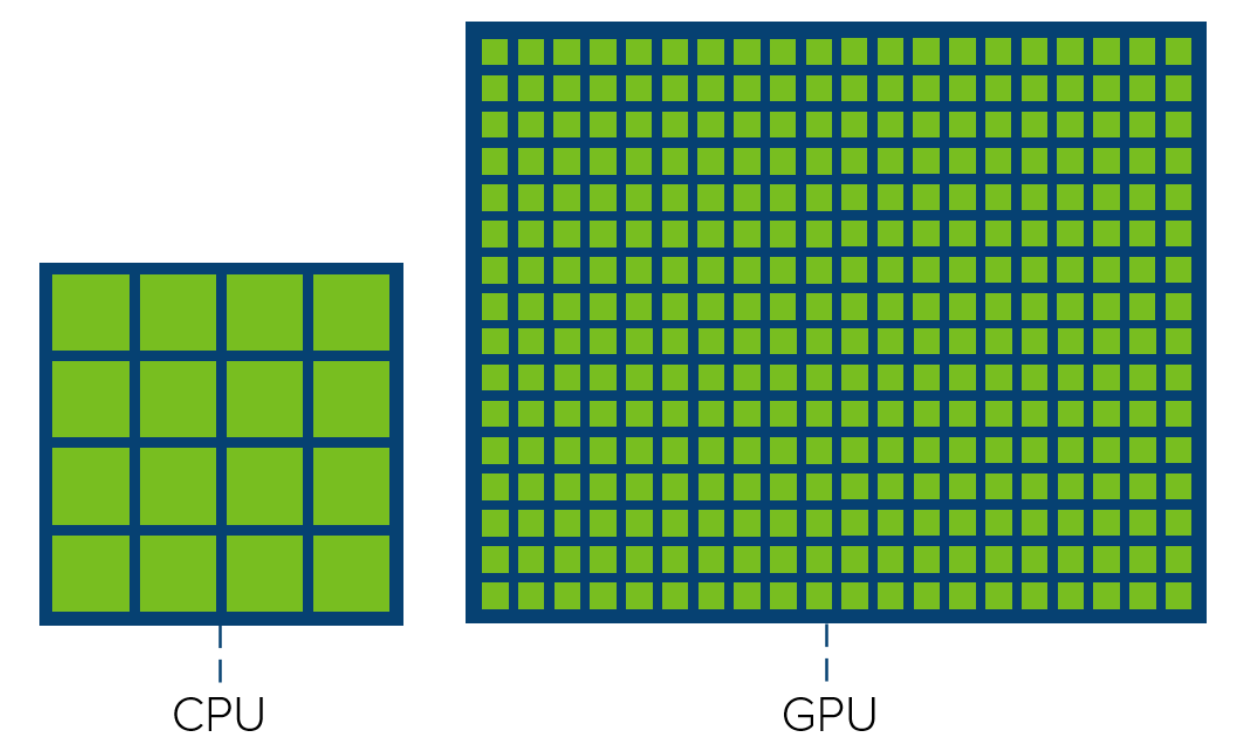
\includegraphics[width=0.9\textwidth]{images/cpuvgpu.png}
    \column{0.5\textwidth}
      \begin{itemize}
        \item Highly parallelisable
        \item Fast communication between operations
        \item GPU 'cores' do less, so no control flow
      \end{itemize}
  \end{columns}
\end{frame}

\begin{frame}[fragile]{JAX numpy vs numpy}
  \begin{columns}
    \column{0.5\textwidth}
    \begin{verbatim}
    import numpy as np
    x = np.arange(10)
    y = np.zeros_like(x)
    for i in range(len(x)):
        y[i] = x[i] * 2
    \end{verbatim}
    \column{0.5\textwidth}
    \begin{verbatim}
    import jax.numpy as jnp
    from jax import vmap
    x = jnp.arange(10)
    def double(v):
        return v * 2
    y = vmap(double)(x)
    \end{verbatim}
  \end{columns}
\end{frame}

\begin{frame}{JAX-based Nested Sampling Integration}
  \begin{columns}
    \column{0.5\textwidth}
      \centering
      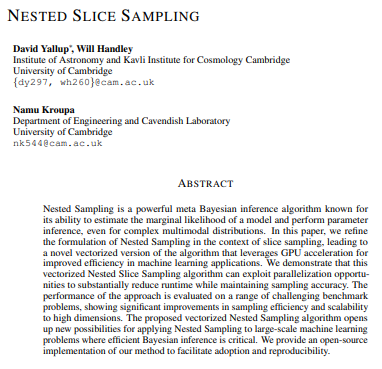
\includegraphics[width=0.8\textwidth]{images/nested_sampling_paper.png}
    \column{0.5\textwidth}
      \begin{itemize}
        \item BlackJAX integration
        \item GPU-accelerated sampling
      \end{itemize}
  \end{columns}
\end{frame}

\section{Fitting SNIa}

\begin{frame}{Standard Likelihood for Supernovae}
  \centering
  For photometric observations with Gaussian uncertainties:
  \begin{equation*}
    \mathcal{L}(\theta) = \prod_{i=1}^{N} \frac{1}{\sqrt{2\pi\sigma_i^2}} \exp\left(-\frac{(f_i^{\text{obs}} - f_i^{\text{model}}(\theta))^2}{2\sigma_i^2}\right)
  \end{equation*}
  \begin{itemize}
    \item $f_i^{\text{obs}}$: observed fluxes
    \item $f_i^{\text{model}}(\theta)$: SALT model fluxes 
    \item $\sigma_i$: flux uncertainties
  \end{itemize}
\end{frame}


\begin{frame}{Standard vs. Anomaly Detection Likelihoods}
  \footnotesize
  \begin{columns}
    \column{0.5\textwidth}
    \textbf{Standard Likelihood:}
    \begin{align}
      \log \mathcal{L}_{\text{std}} &= -\frac{1}{2}\sum_i \left(\frac{f_i - m_i}{\sigma_i}\right)^2 \nonumber \\
      &\quad - \frac{1}{2}\sum_i \log(2\pi\sigma_i^2)
    \end{align}
    \begin{itemize}
      \item $f_i$: Observed flux
      \item $m_i$: Model flux (SALT3)
      \item $\sigma_i$: Flux uncertainty
    \end{itemize}
    
    \column{0.5\textwidth}
    \textbf{Anomaly Detection Likelihood:}
    \begin{align}
      \log \mathcal{L}_{\text{anom}} &= \sum_i \begin{cases}
        \log \mathcal{L}_i + \log(1-p), & e_i^{\max} \\
        \log p - \log \Delta, & \text{else}
      \end{cases}
    \end{align}
    \begin{itemize}
      \item $\log \mathcal{L}_i$: Point-wise likelihood
      \item $p$: Anomaly probability 
      \item $e_i^{\max}$: Boolean for normal data
      \item $\Delta$: Maximum flux range
    \end{itemize}
  \end{columns}
  
\end{frame}

\begin{frame}{Automated Bandpass Selection Results}
  \begin{columns}
    \column{0.5\textwidth}
      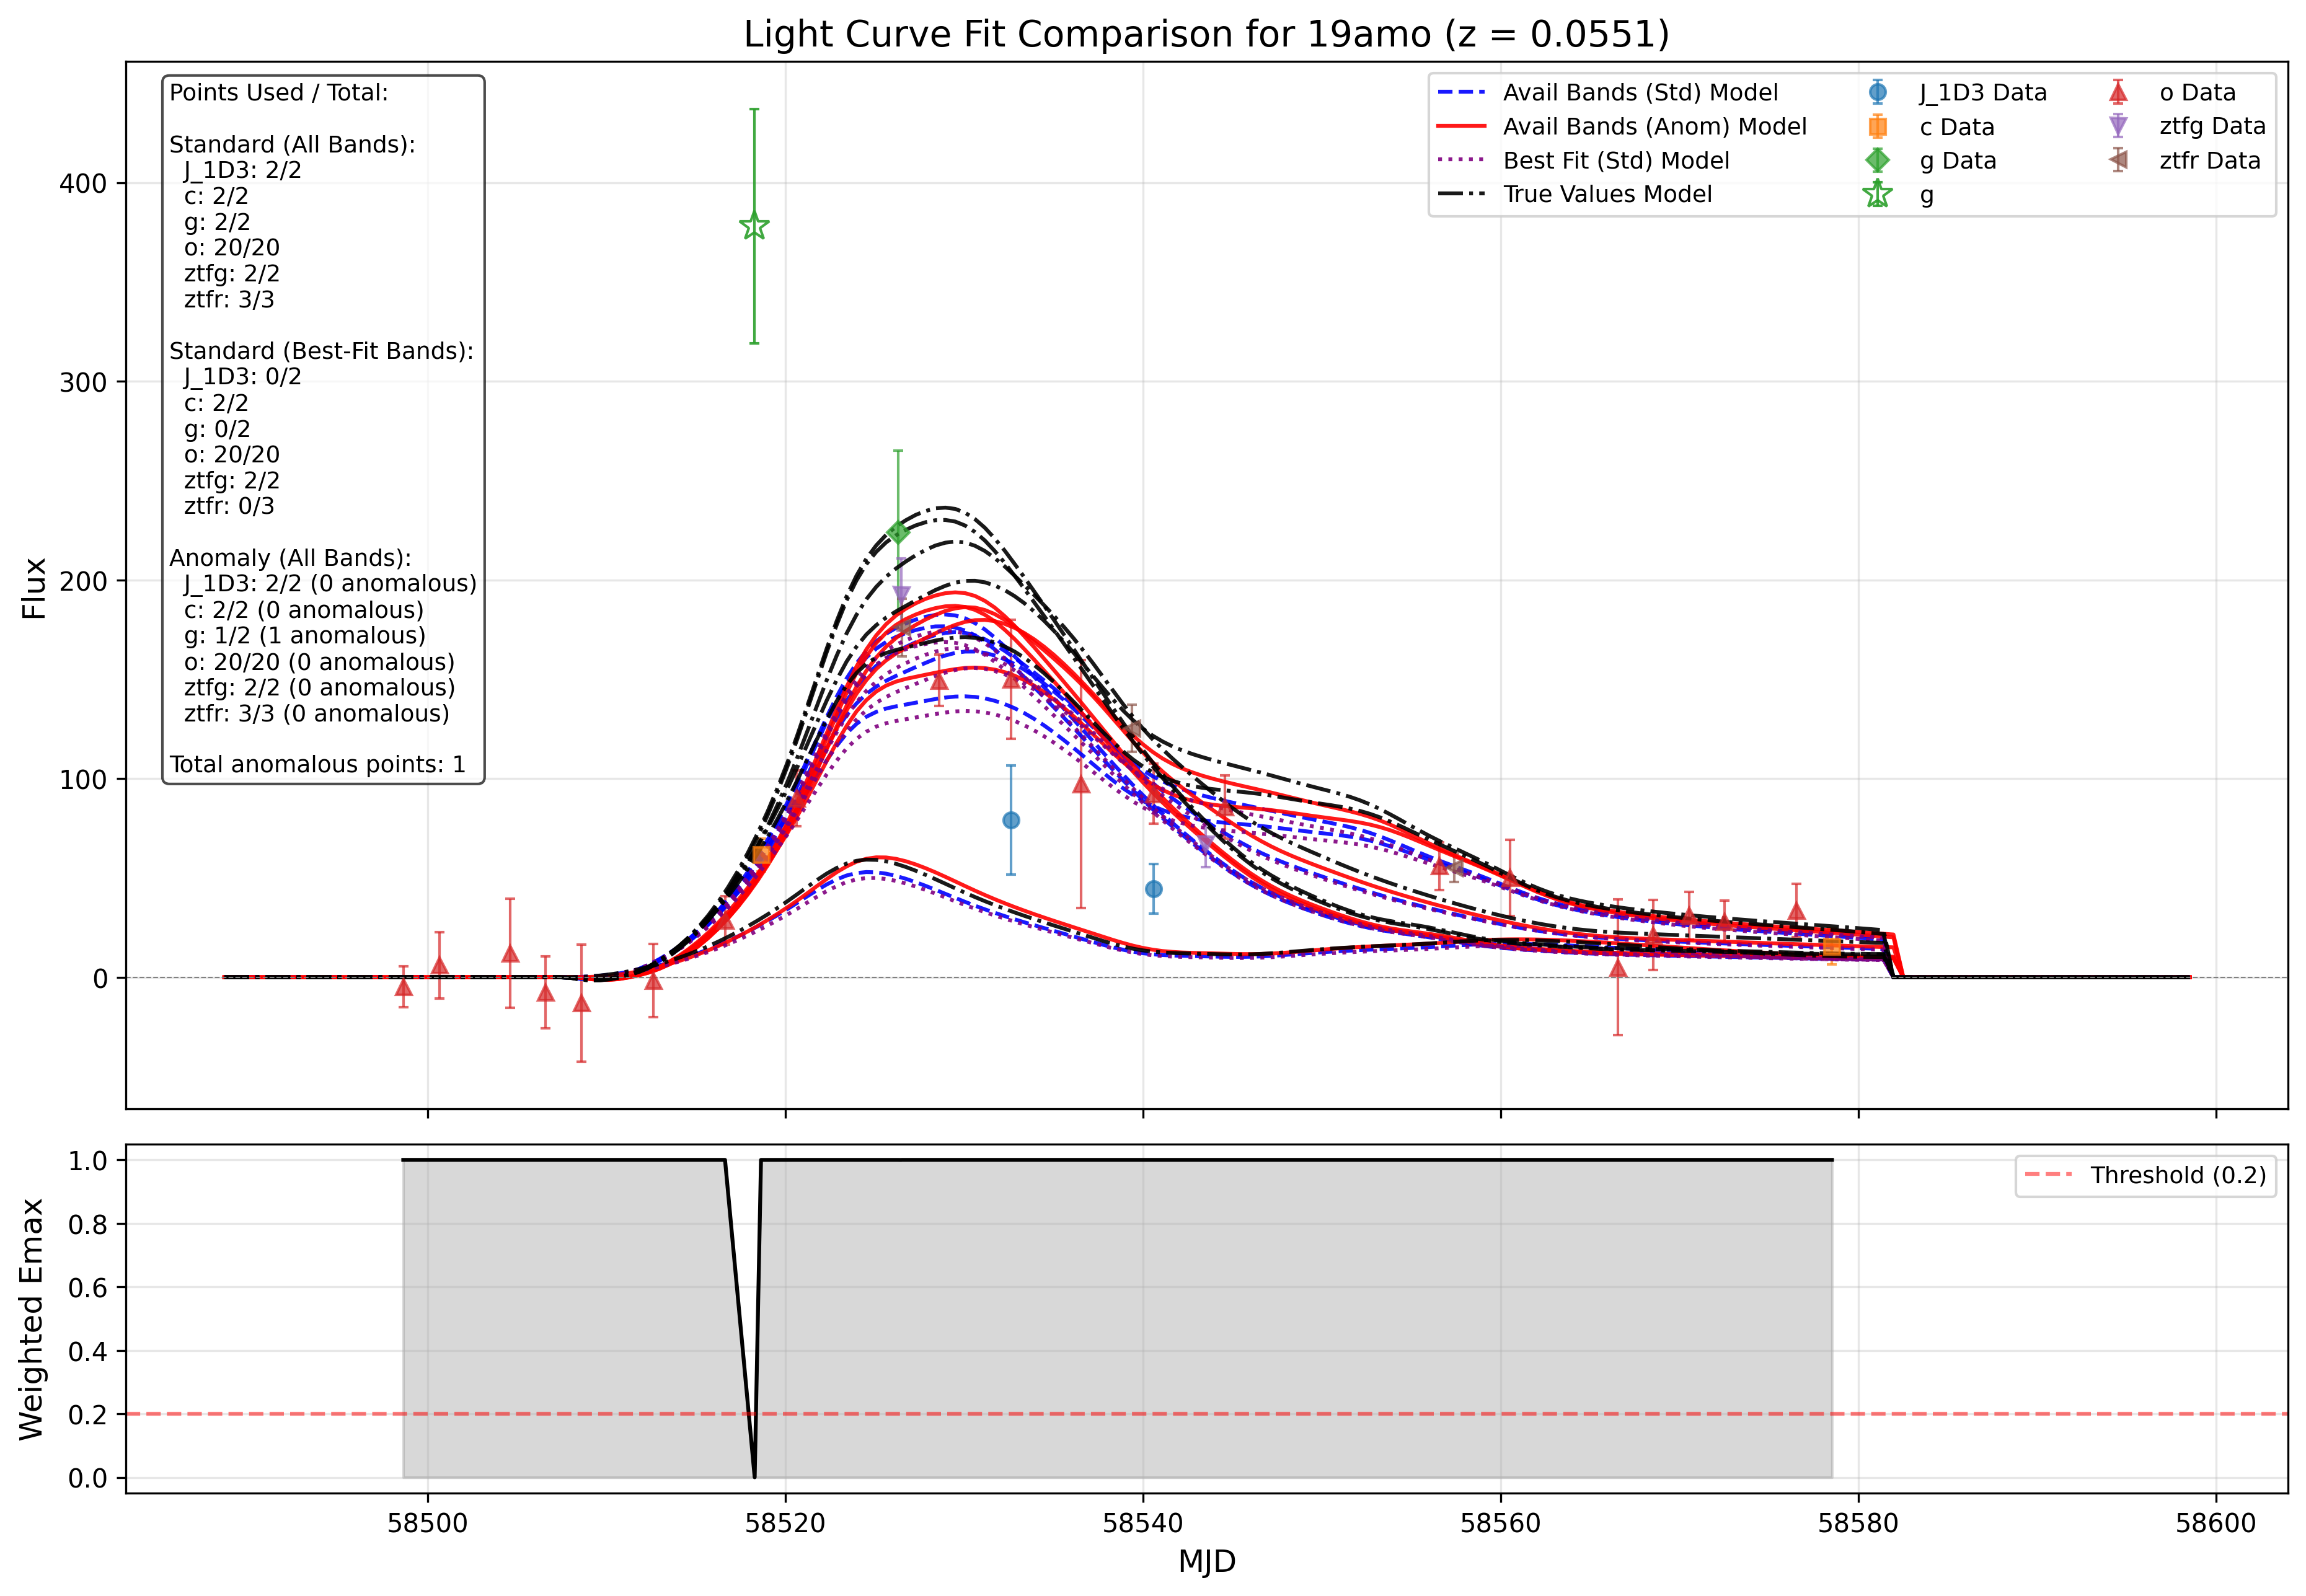
\includegraphics[width=1\textwidth]{images/light_curve_comparison_19amo.png}
    \column{0.5\textwidth}
      \textbf{Our method demonstrates:}
      \begin{enumerate}
        \item Standard flagging
        \item Automatic filter selection
        \item Data preservation
      \end{enumerate}
  \end{columns}
\end{frame}

\begin{frame}{SN 19amo: Classic 'anomaly detection' example}
  \begin{columns}
    \column{0.5\textwidth}
    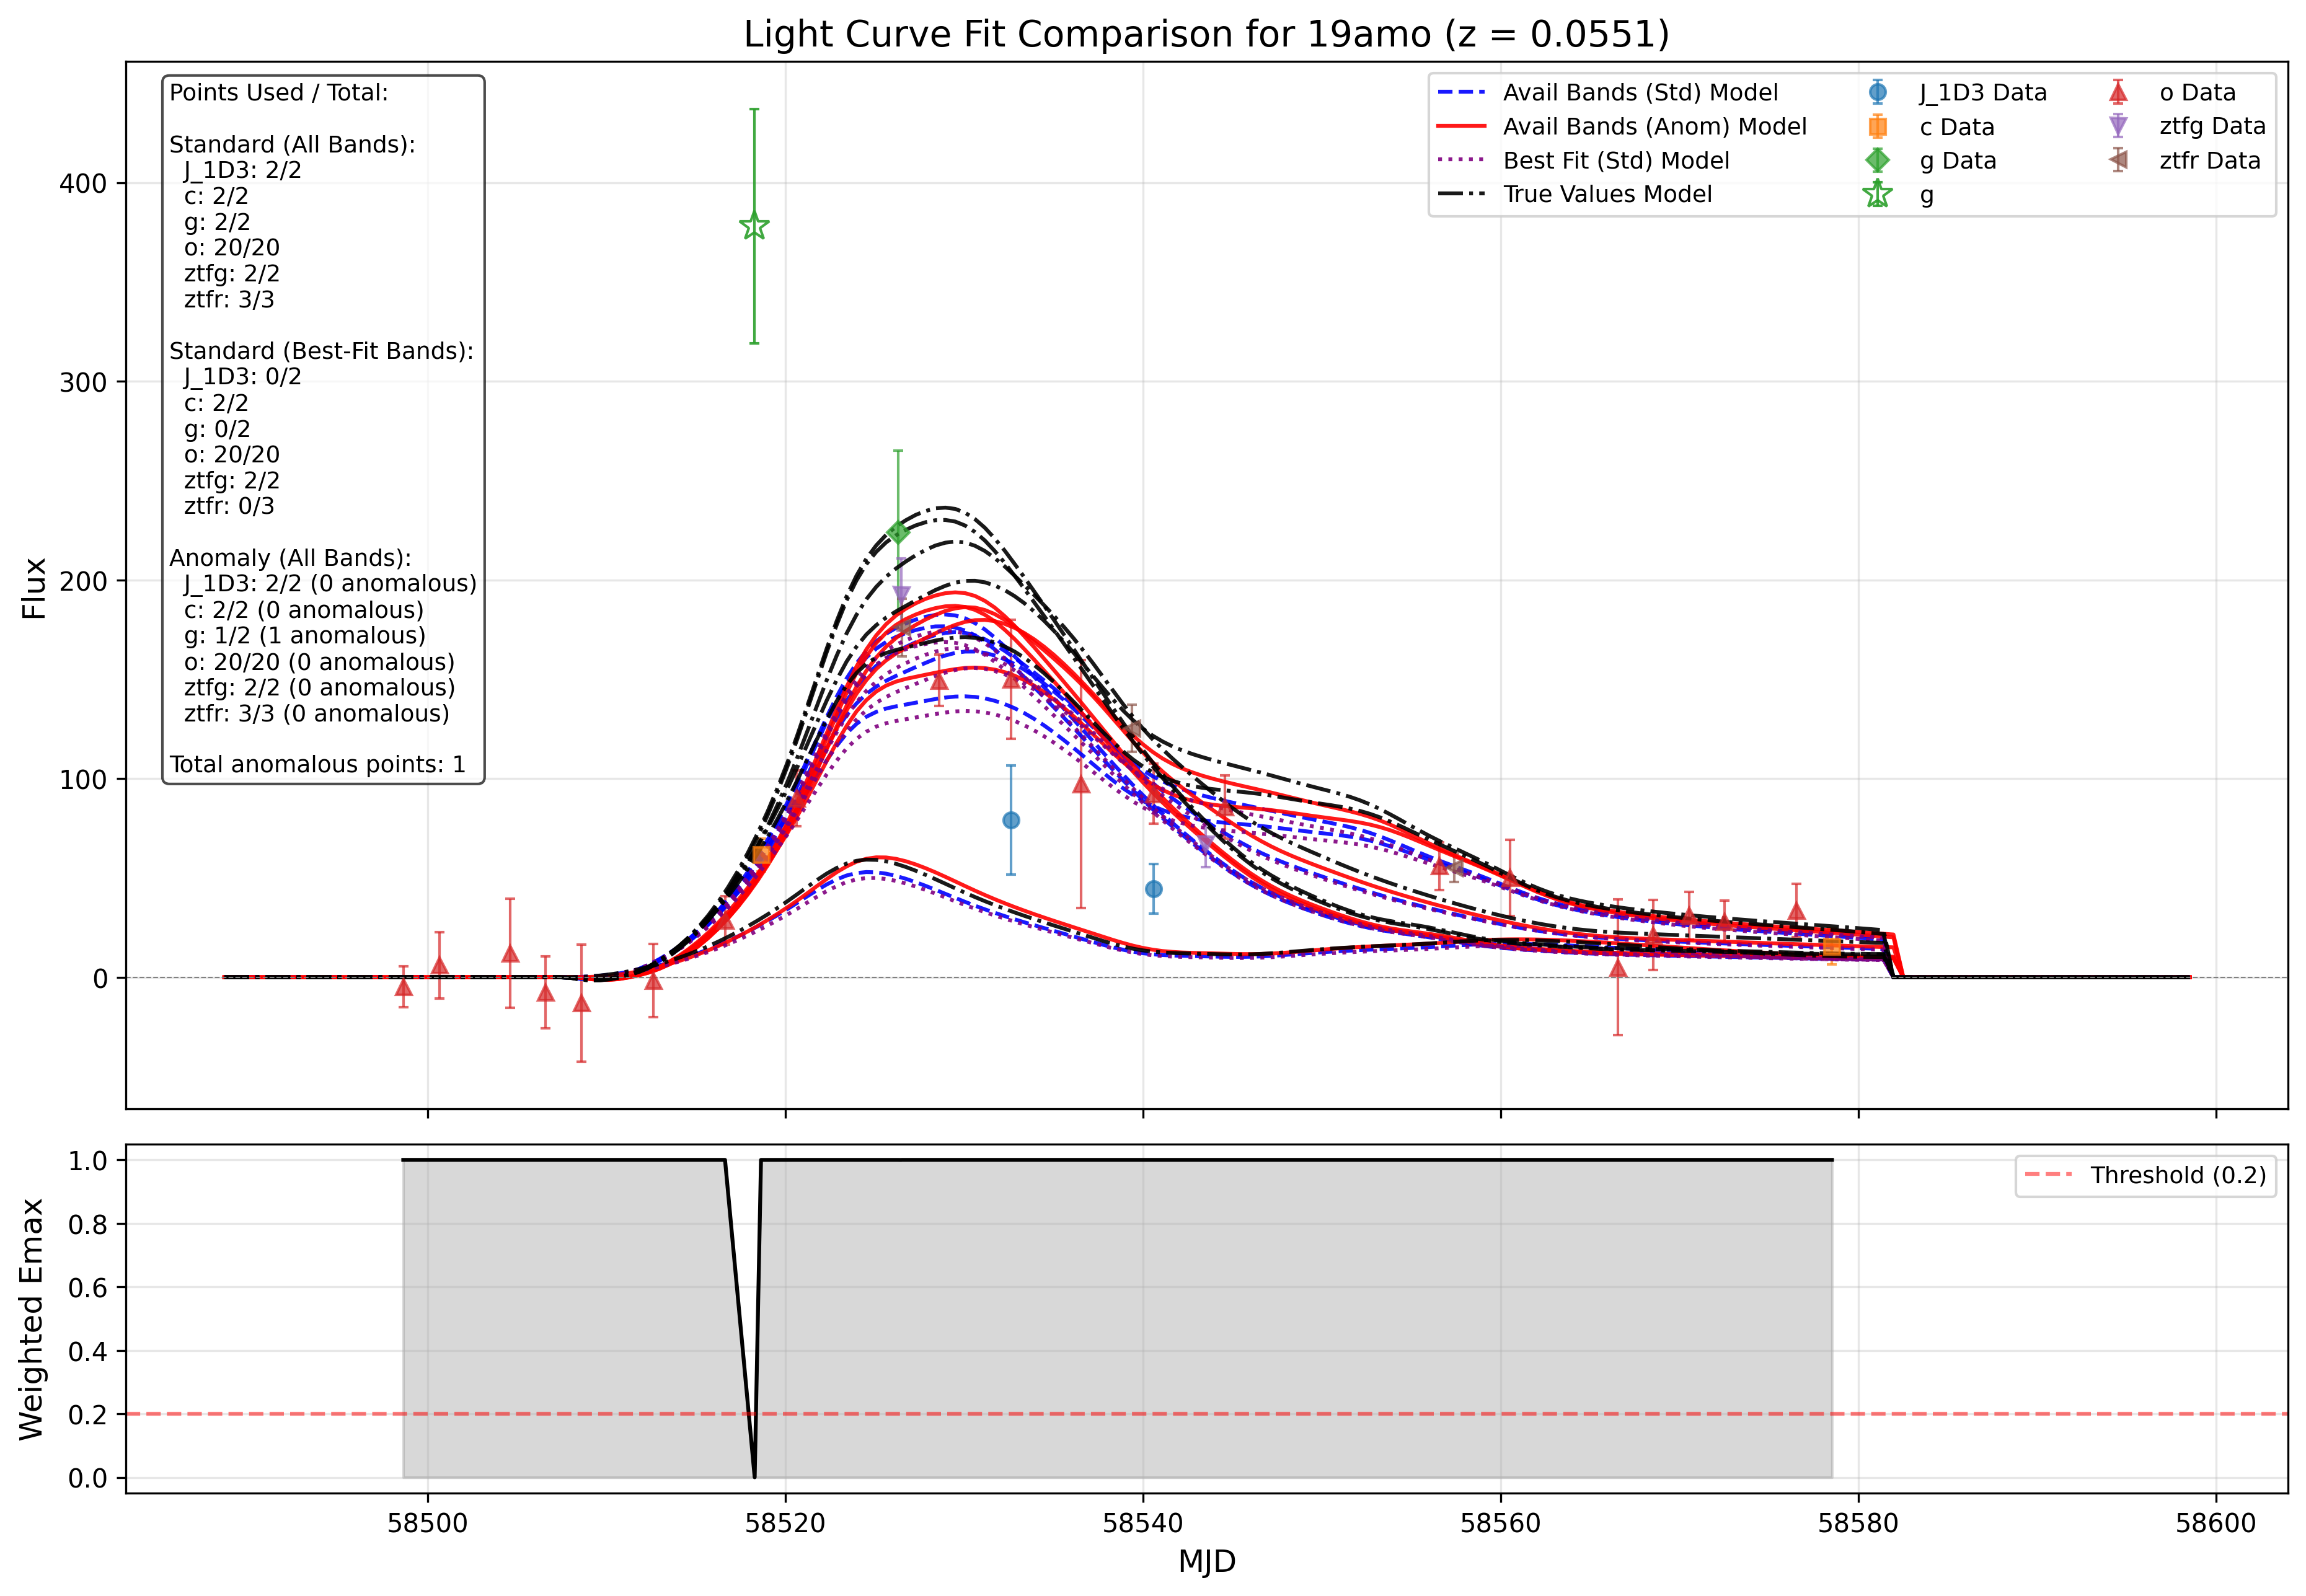
\includegraphics[width=1\textwidth]{images/light_curve_comparison_19amo.png}
    \column{0.5\textwidth}
    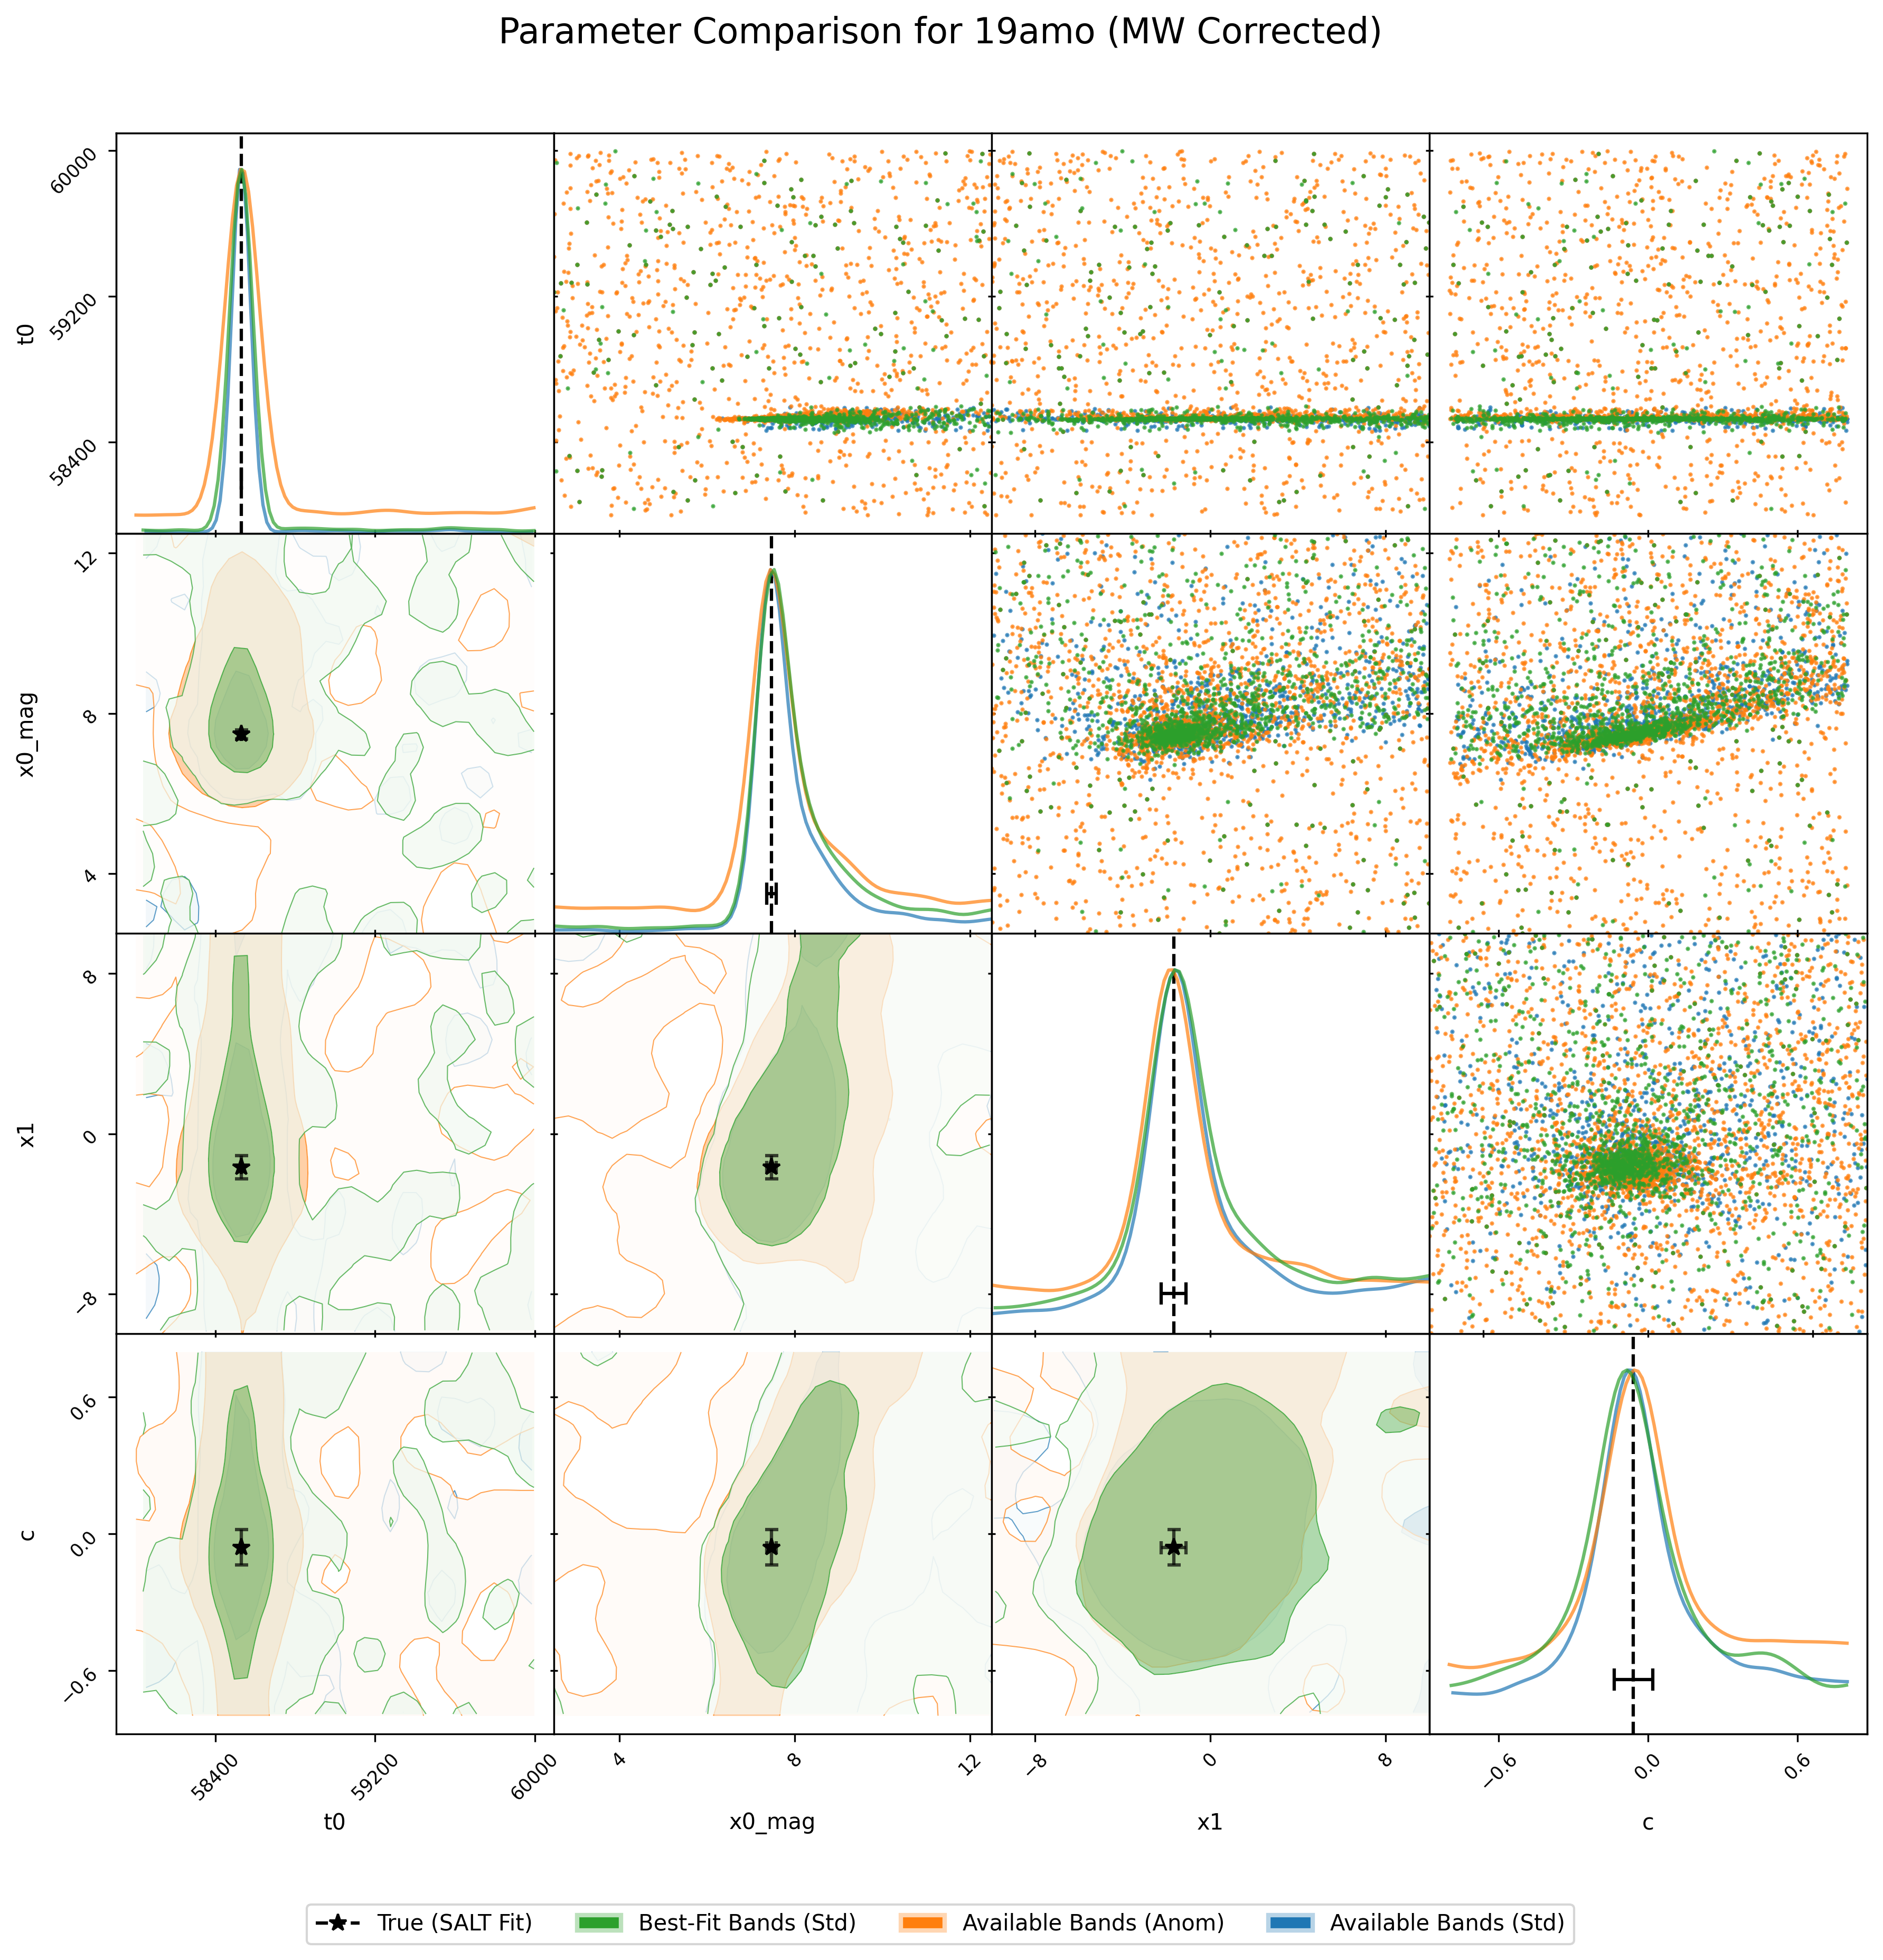
\includegraphics[width=1\textwidth]{images/corner_comparison_19amo.png}
  \end{columns}
\end{frame}

\begin{frame}{SN 19vnk: Automatic filter removal}
  \begin{columns}
    \column{0.5\textwidth}
    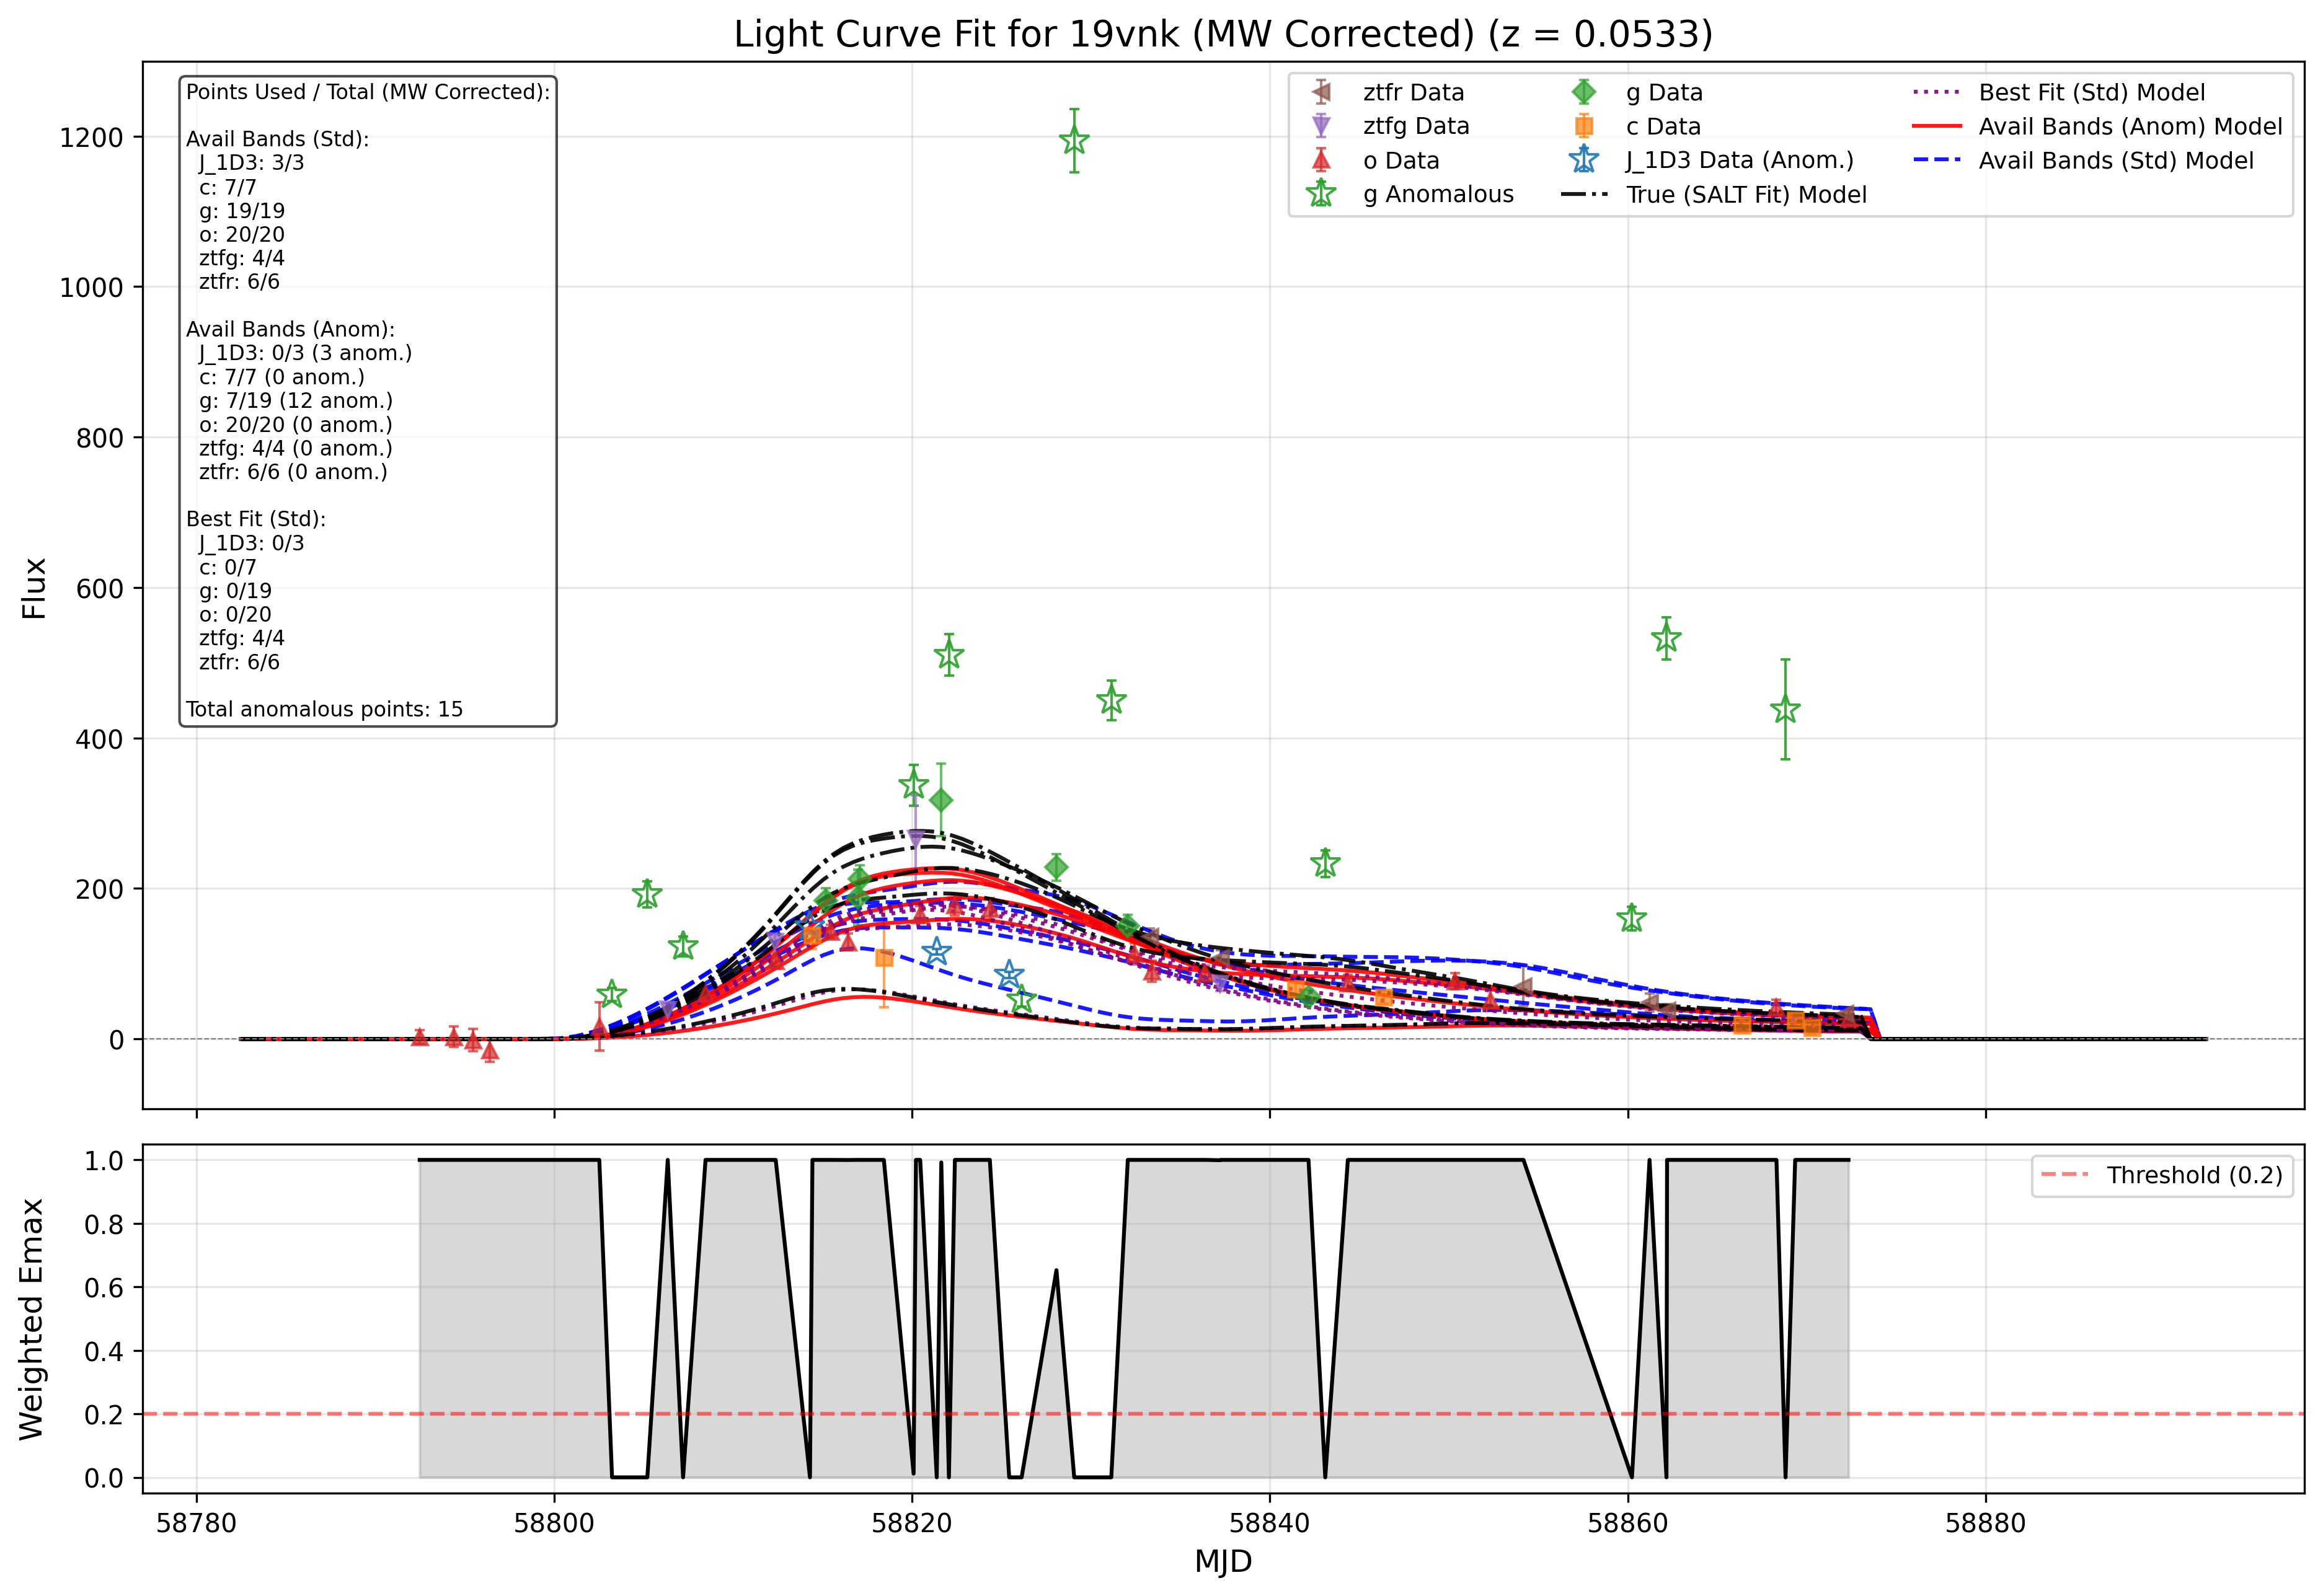
\includegraphics[width=1\textwidth]{images/light_curve_comparison_19vnk.png}
    \column{0.5\textwidth}
    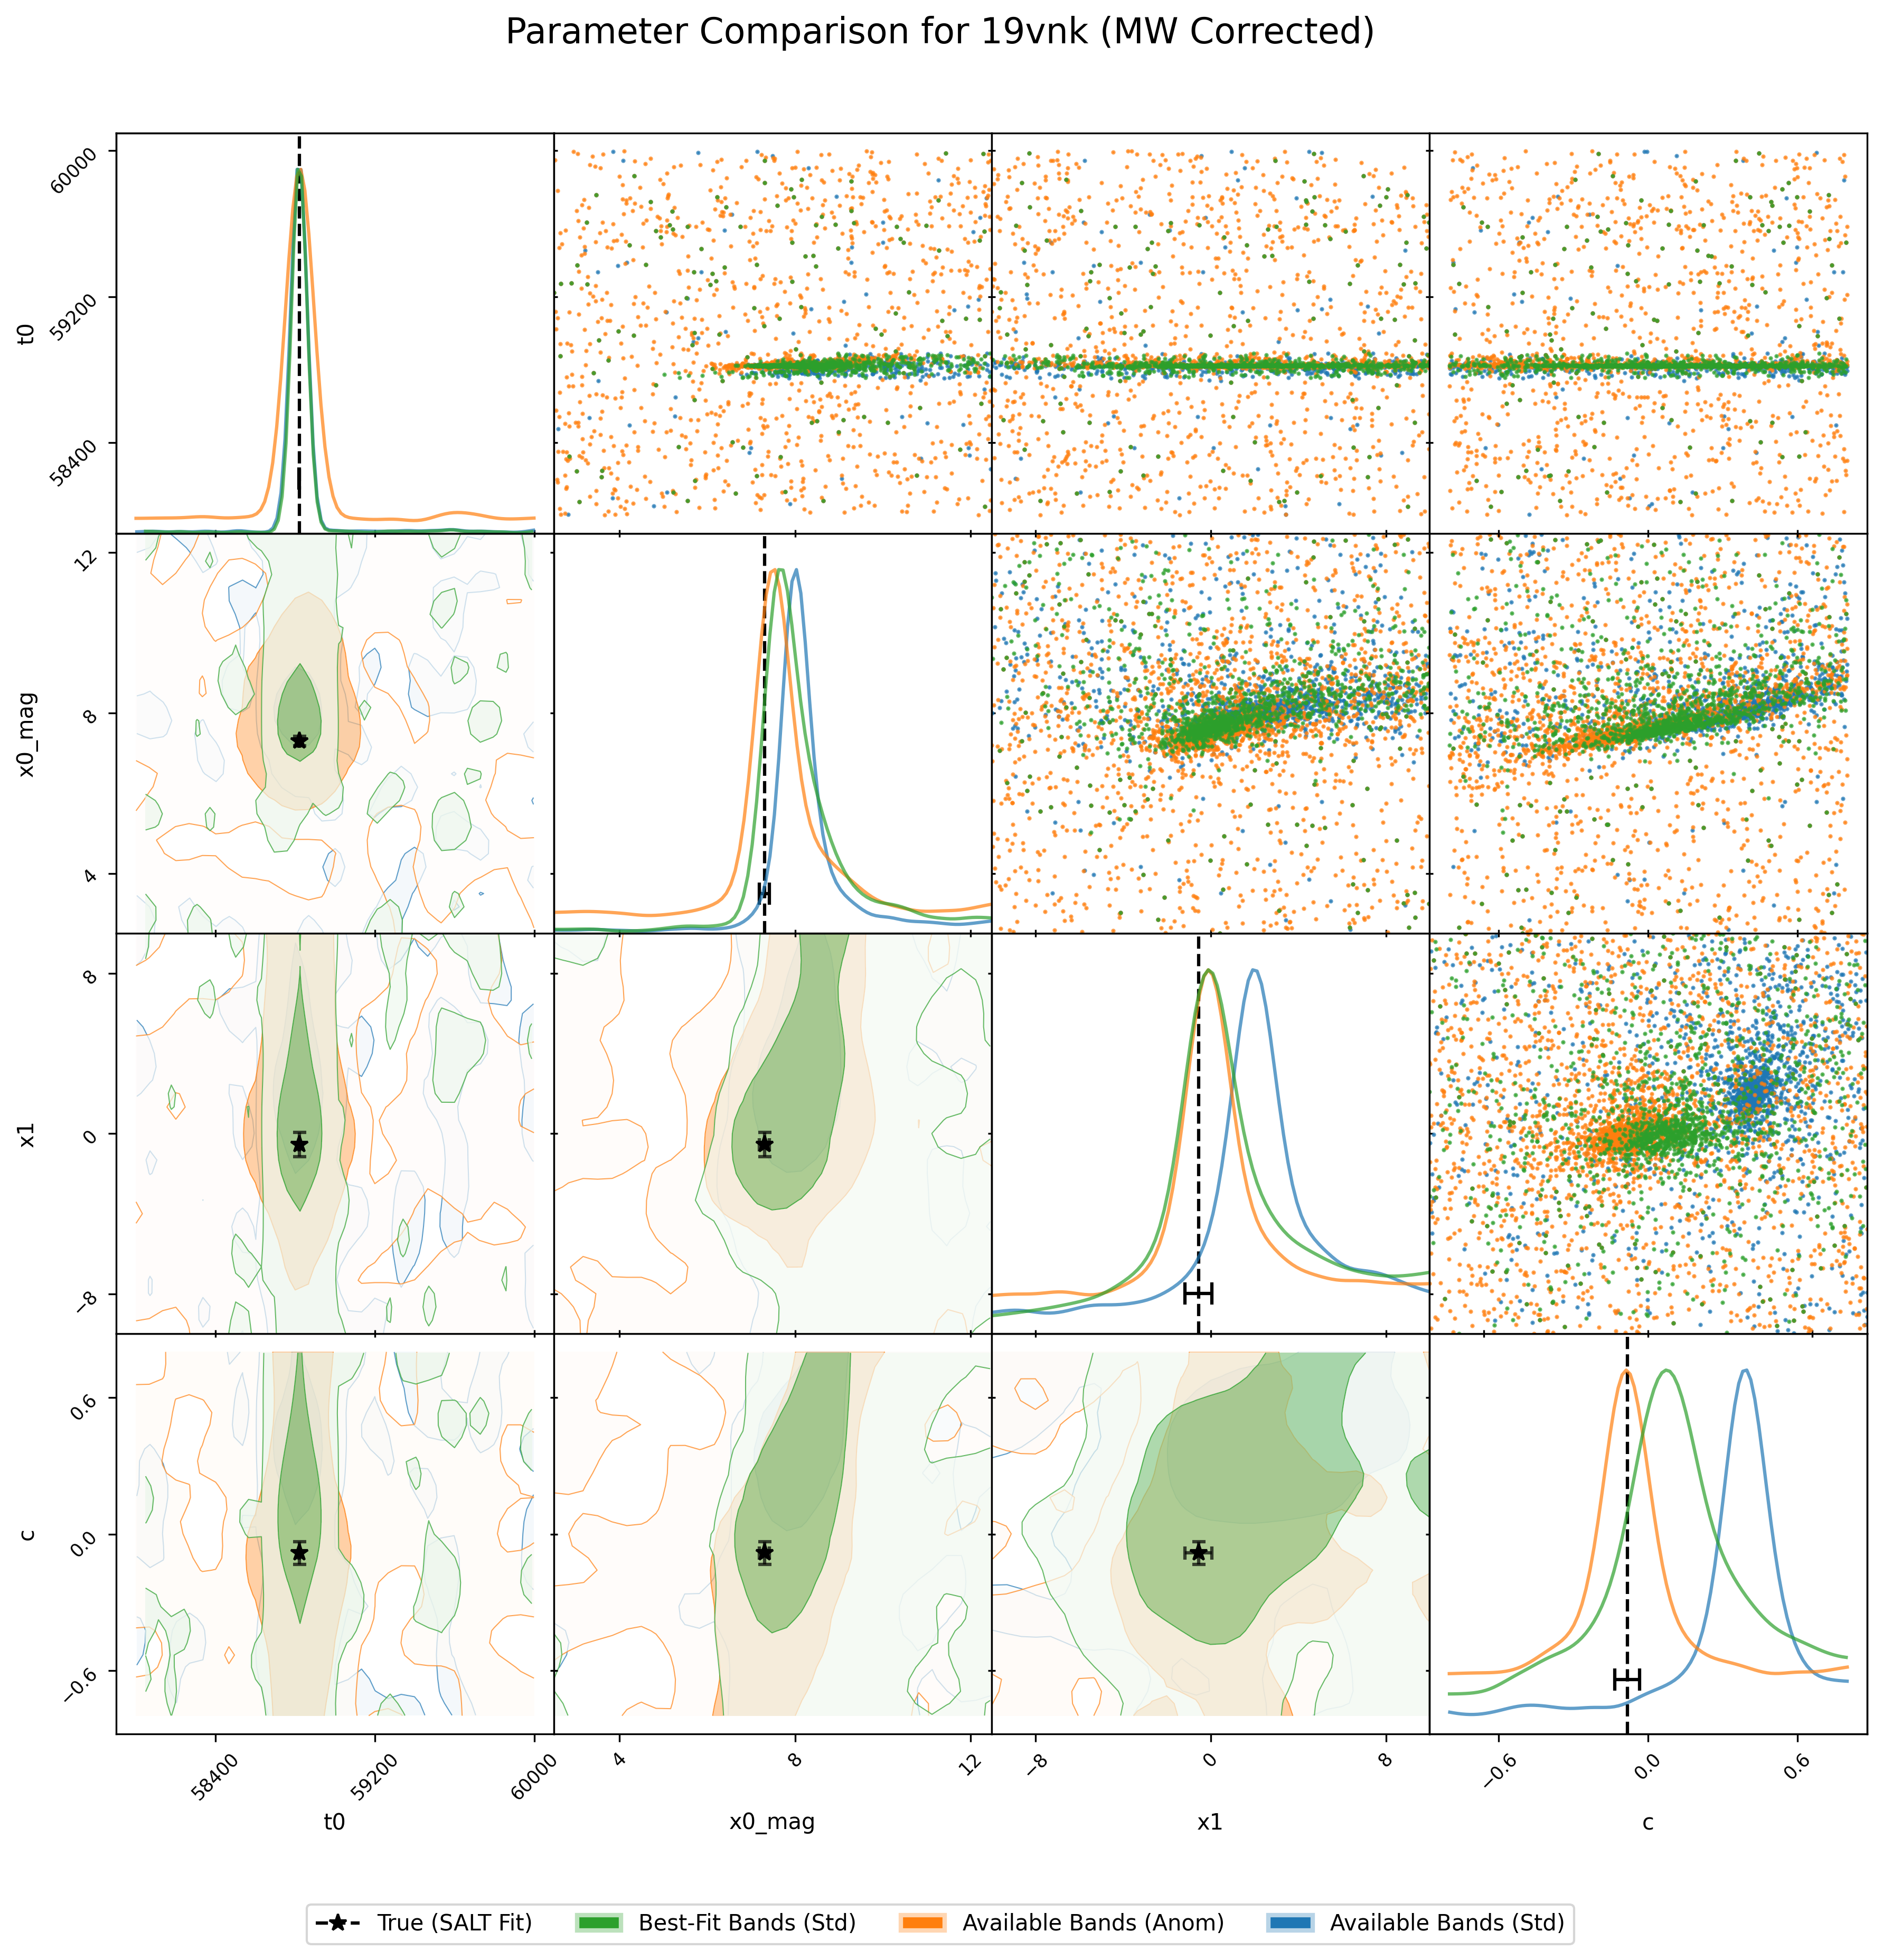
\includegraphics[width=1\textwidth]{images/corner_comparison_19vnk.png}
  \end{columns}
\end{frame}

\begin{frame}{SN 19kai: Flagging while preserving some data}
  \begin{columns}
    \column{0.5\textwidth}
    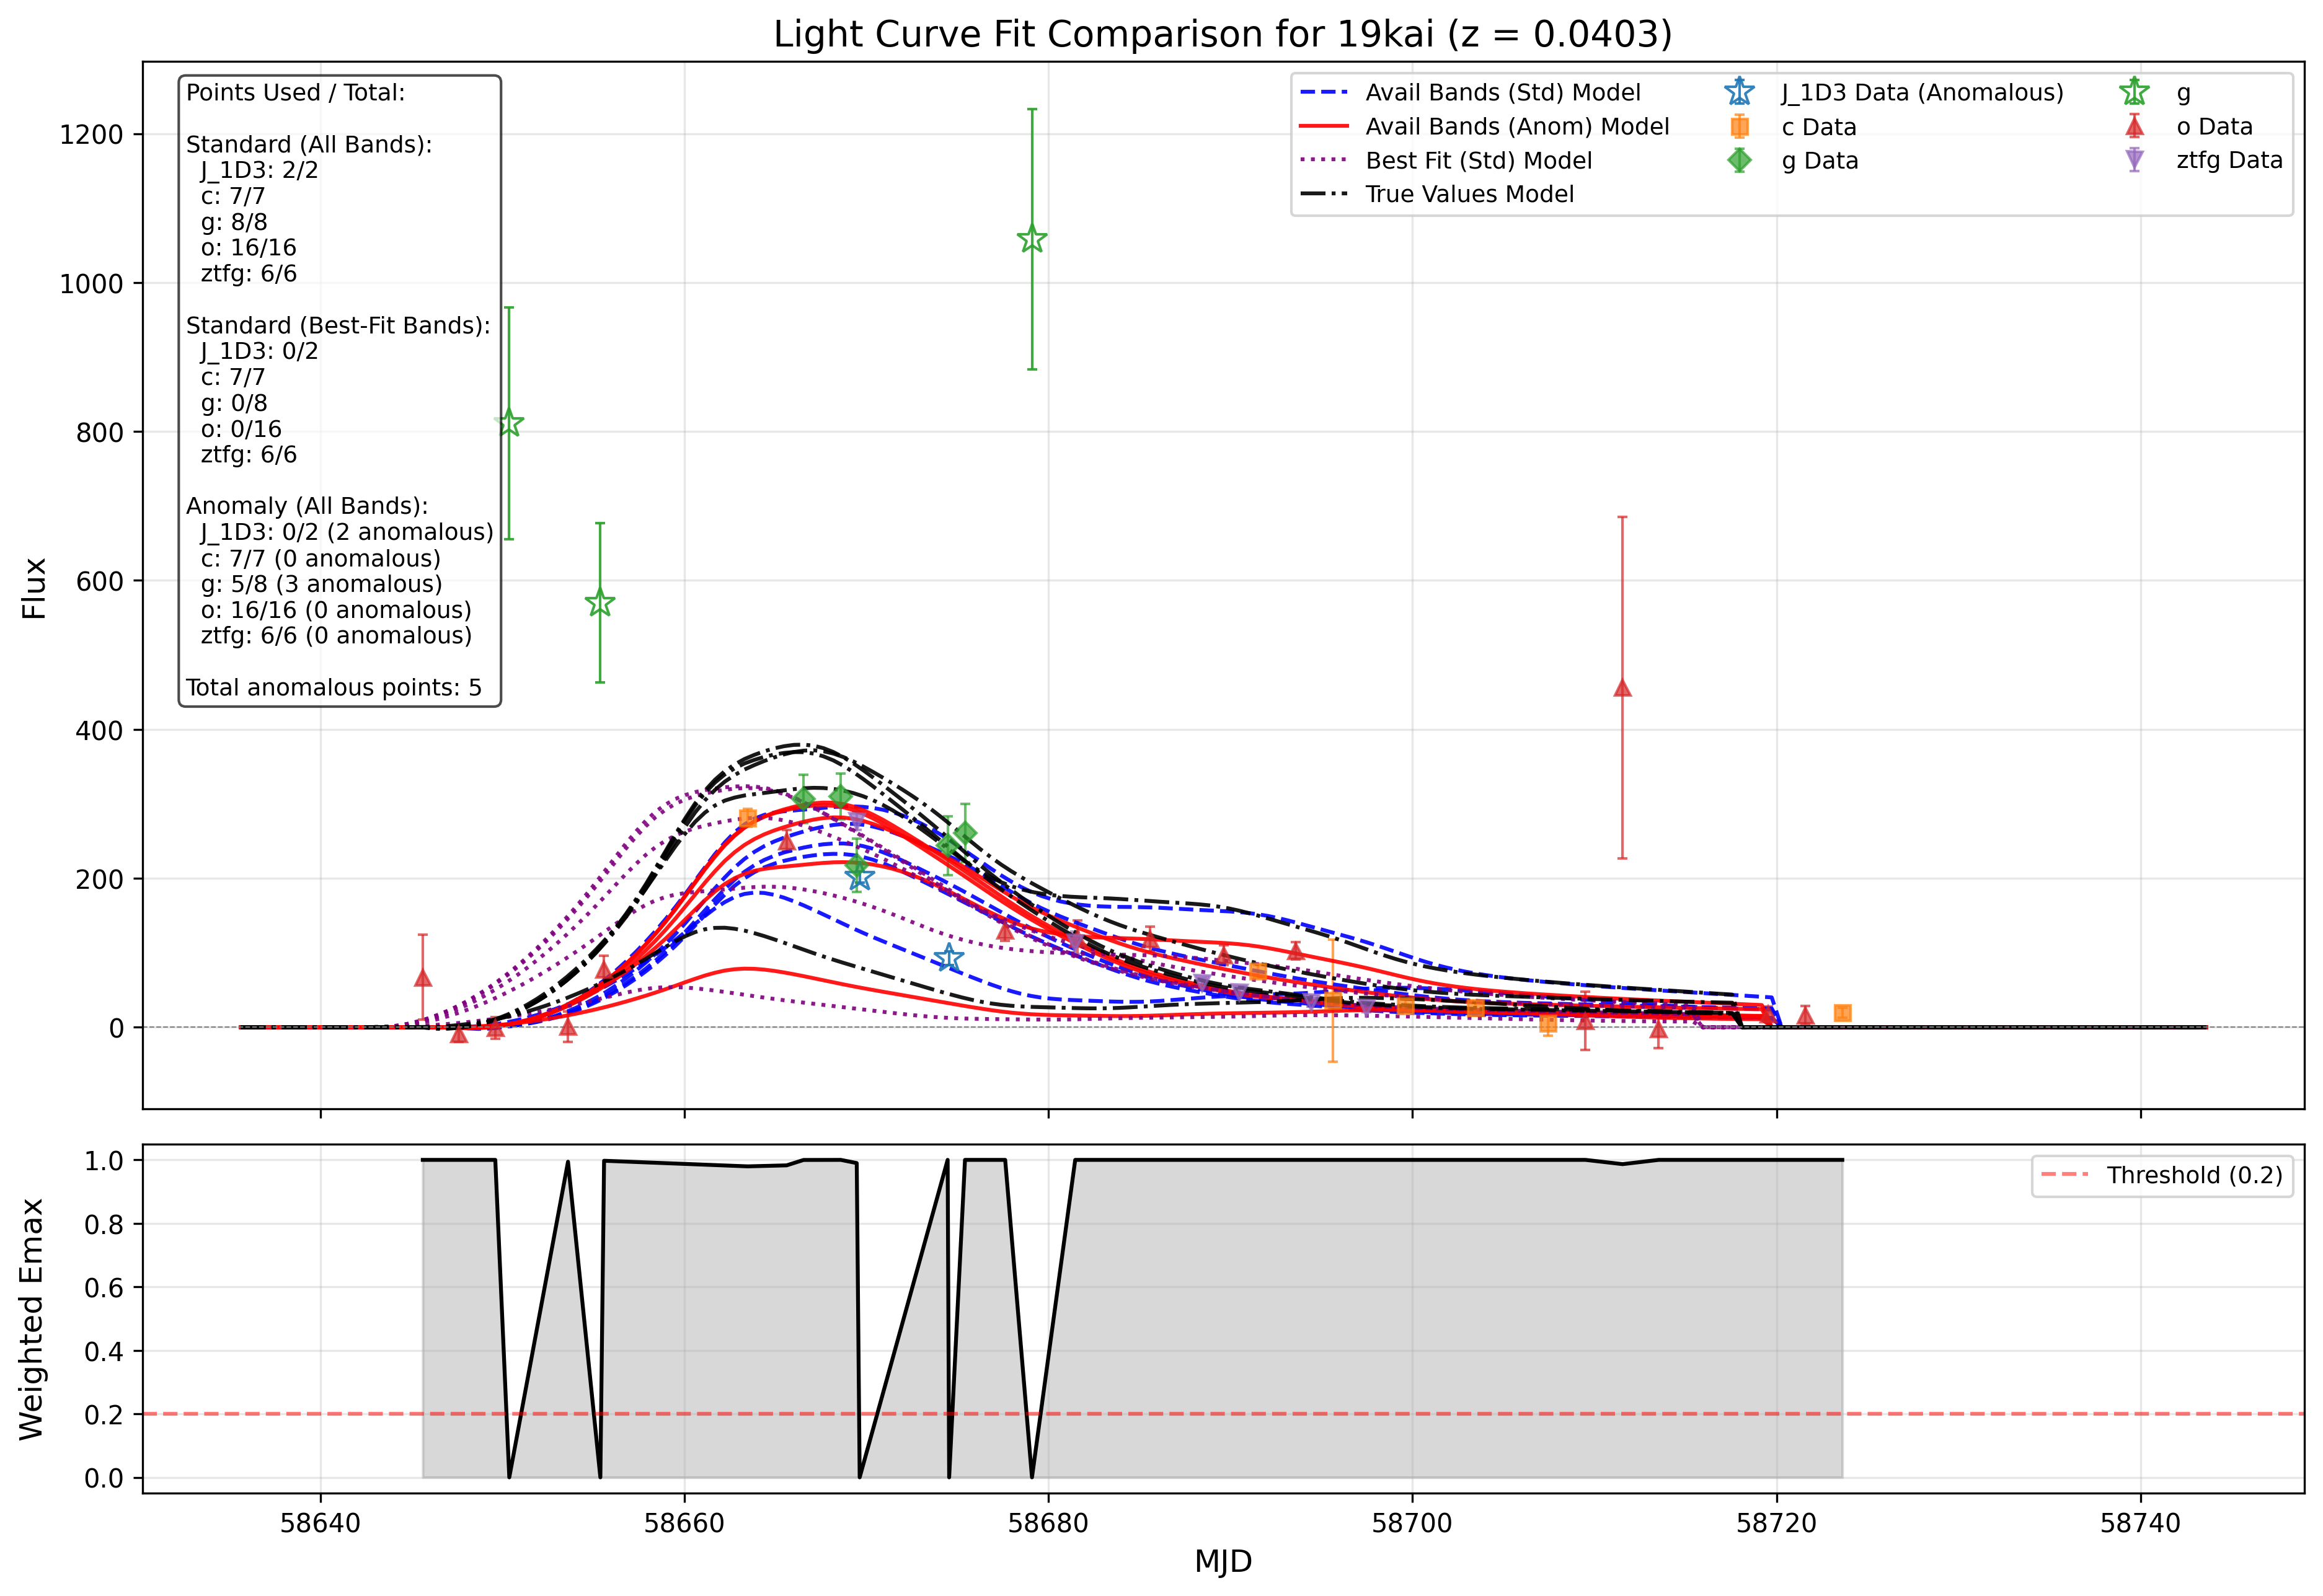
\includegraphics[width=1\textwidth]{images/light_curve_comparison_19kai.png}
    \column{0.5\textwidth}
    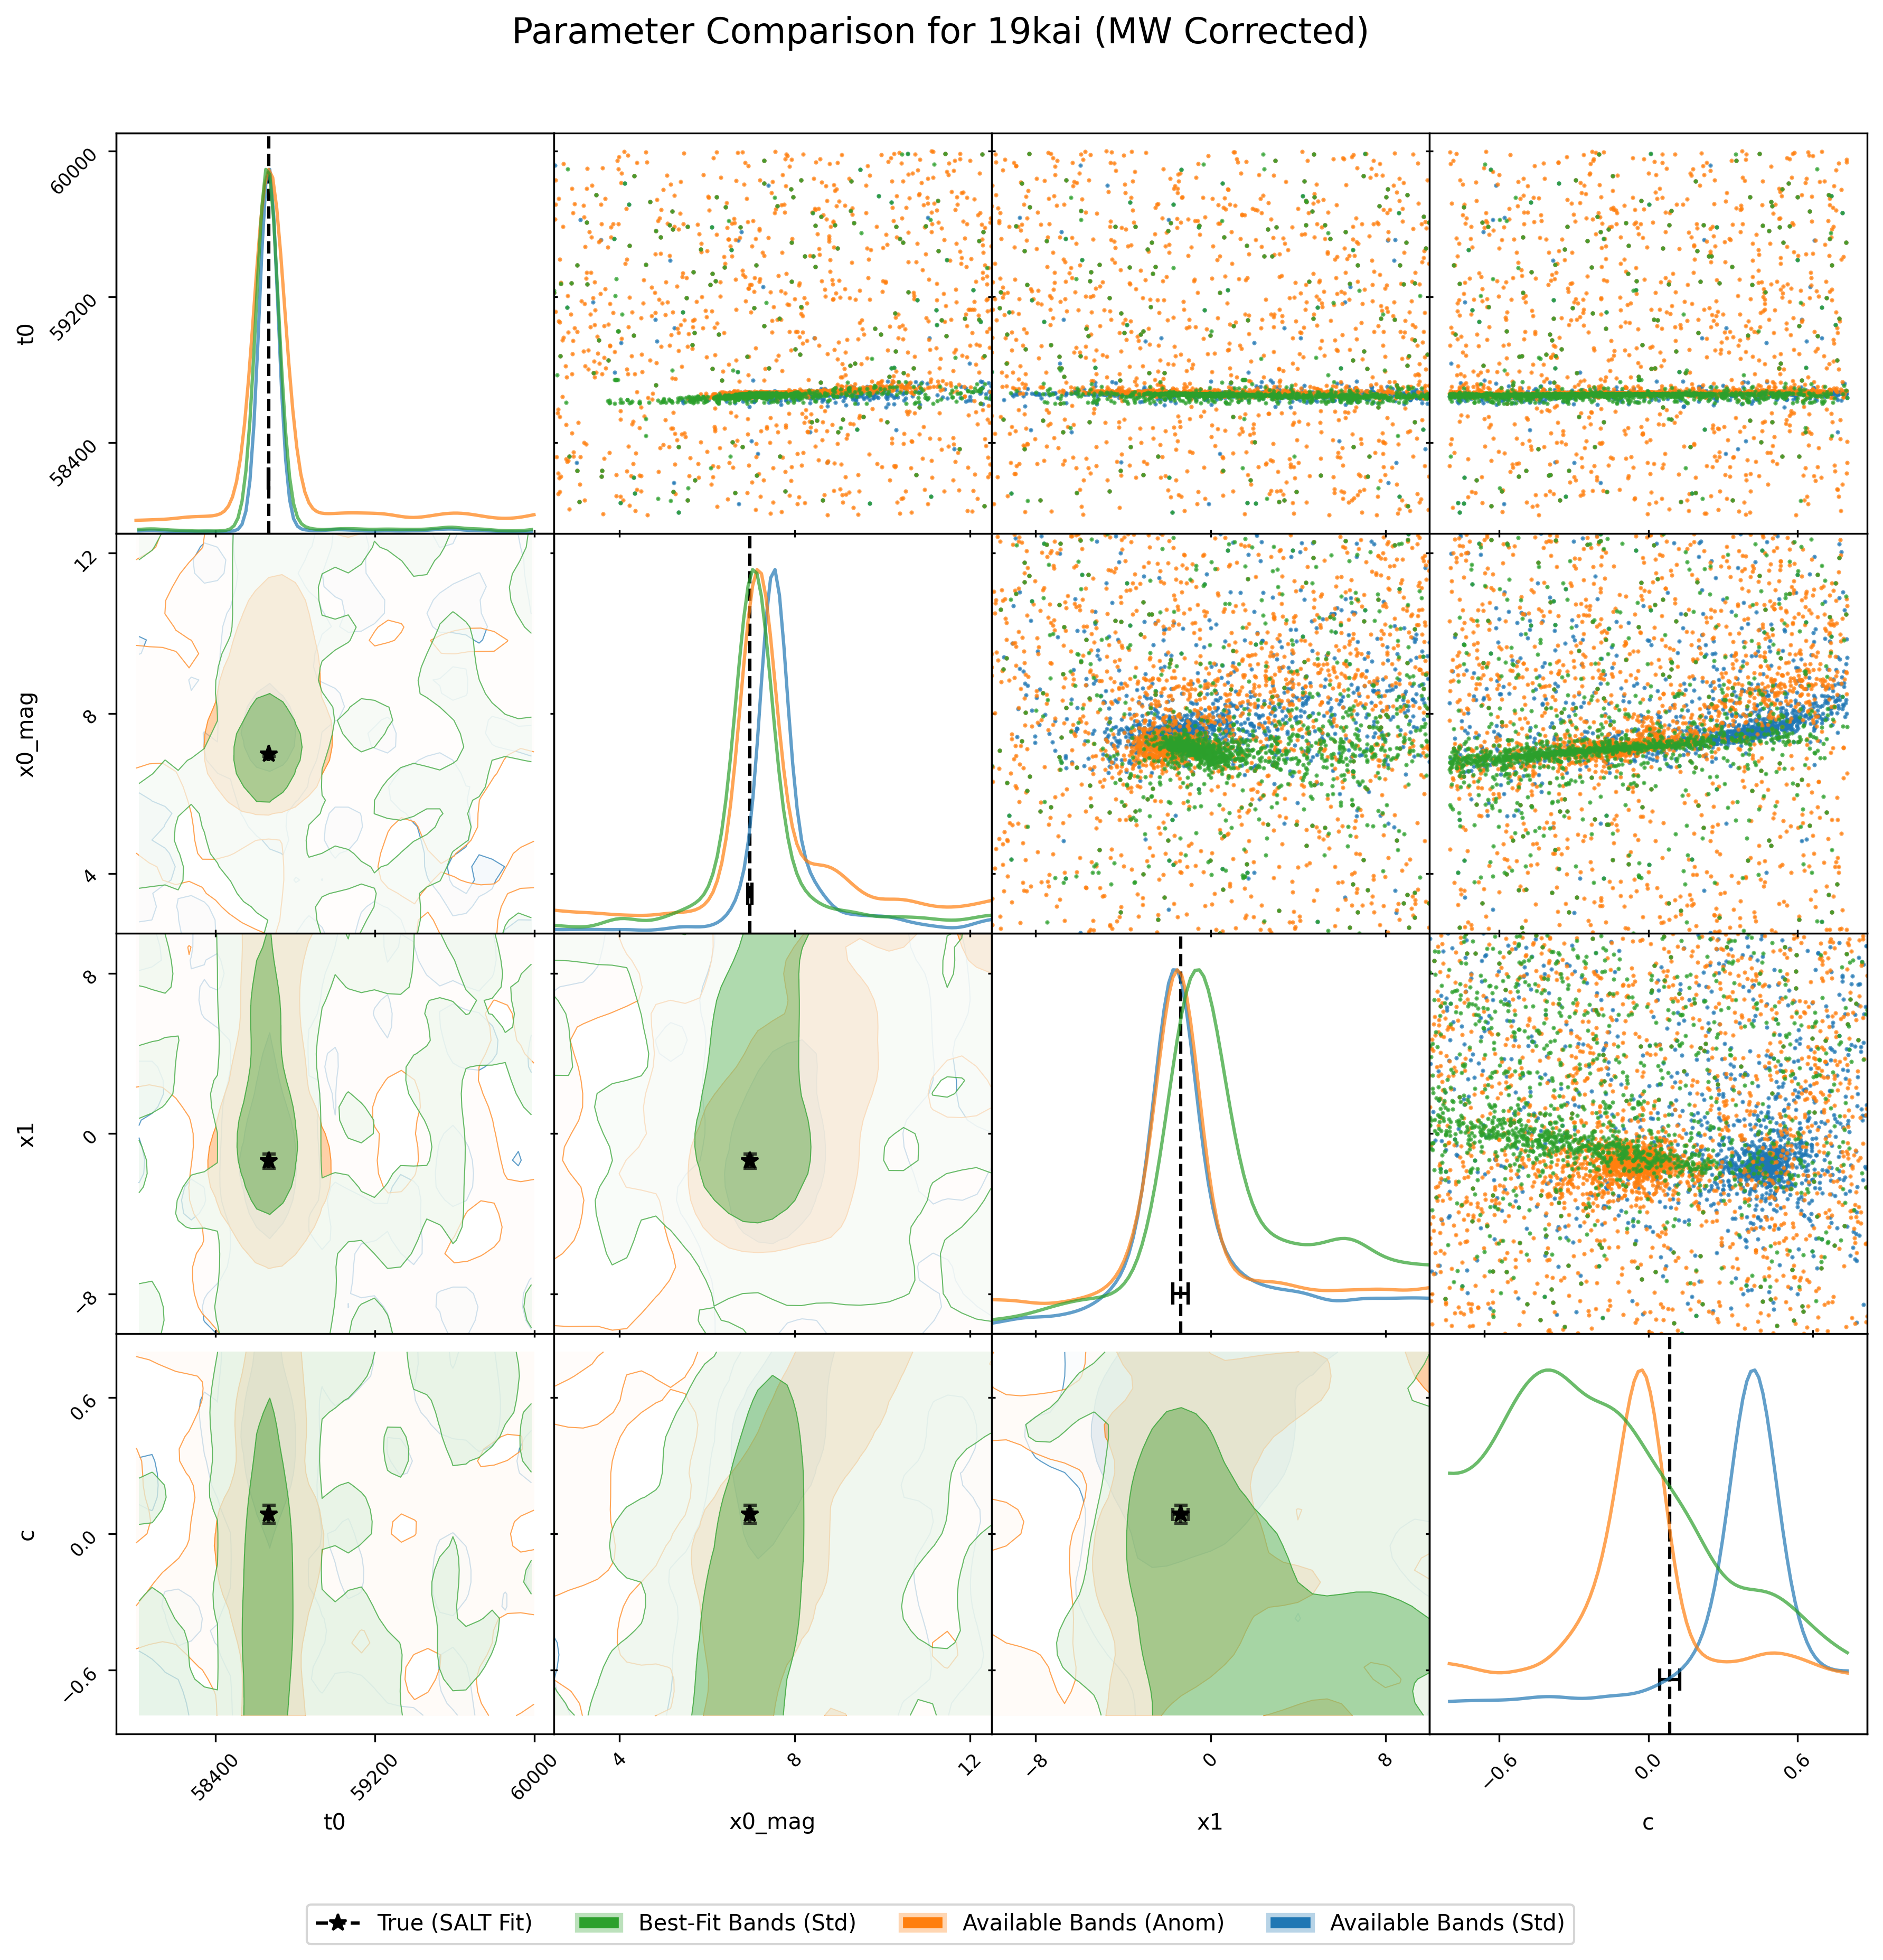
\includegraphics[width=1\textwidth]{images/corner_comparison_19kai.png}
  \end{columns}
\end{frame}

\begin{frame}{Key points}
  \begin{enumerate}
    \item Standard flagging.
    \item Automated filter selection.
    \item Data preservation from previously discarded filters.
  \end{enumerate}
\end{frame}

\begin{frame}{Next steps}
  \begin{enumerate}
    \item \textbf{Distance calibration}
      \begin{itemize}
        \item Improve calibration accuracy using anomaly-aware methods
        \item Better handling of systematic uncertainties in distance measurements
      \end{itemize}
    \item \textbf{H$_0$ measurements}
      \begin{itemize}
        \item Apply to infer H$_0$ 
        \item More robust parameter estimation for cosmological inference
      \end{itemize}
    \item \textbf{More datasets}
      \begin{itemize}
        \item Extend to larger supernova surveys (LSST, Roman Space Telescope)
        \item Apply to different astronomical transients and surveys
      \end{itemize}
  \end{enumerate}
\end{frame}

\begin{frame}{SALT vs SALT + anomaly detection}
  \centering
  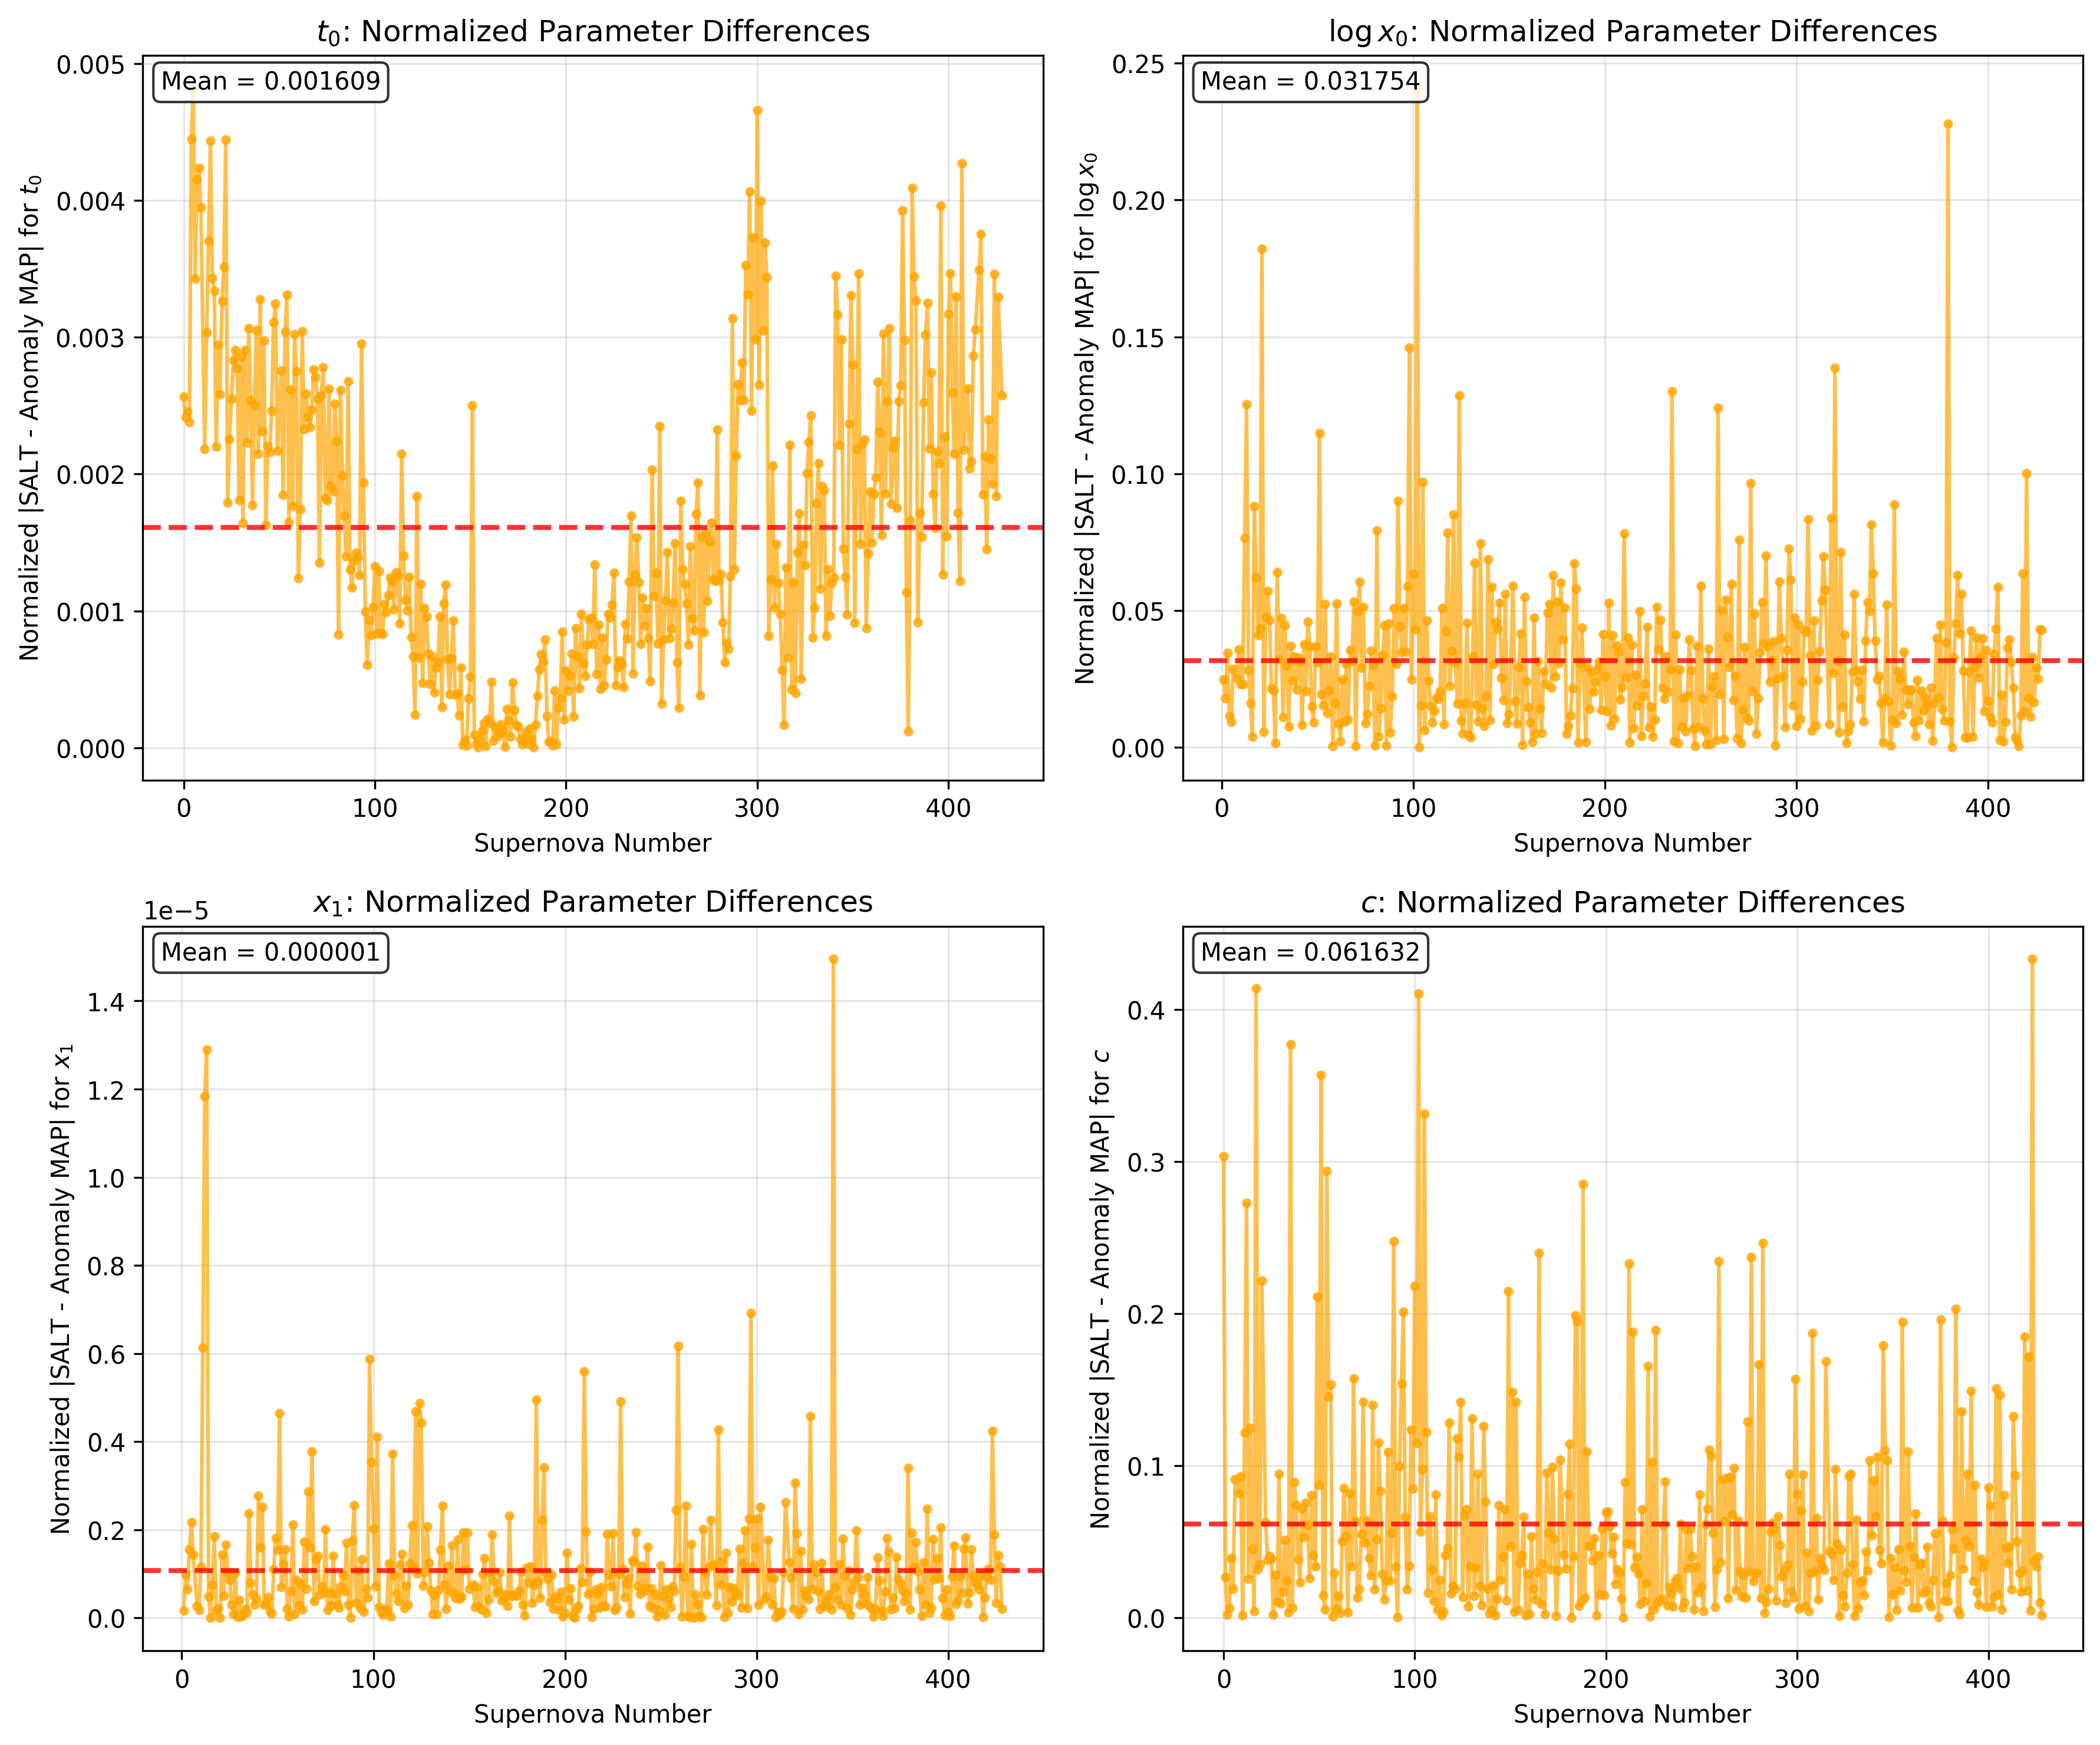
\includegraphics[width=0.6\textwidth]{images/salt_vs_anomaly_map_comparison_Ia_all.png}
\end{frame}

\begin{frame}{Bayesian anomaly detection in other fields}
  \begin{columns}
    \column{0.5\textwidth}
    \centering
    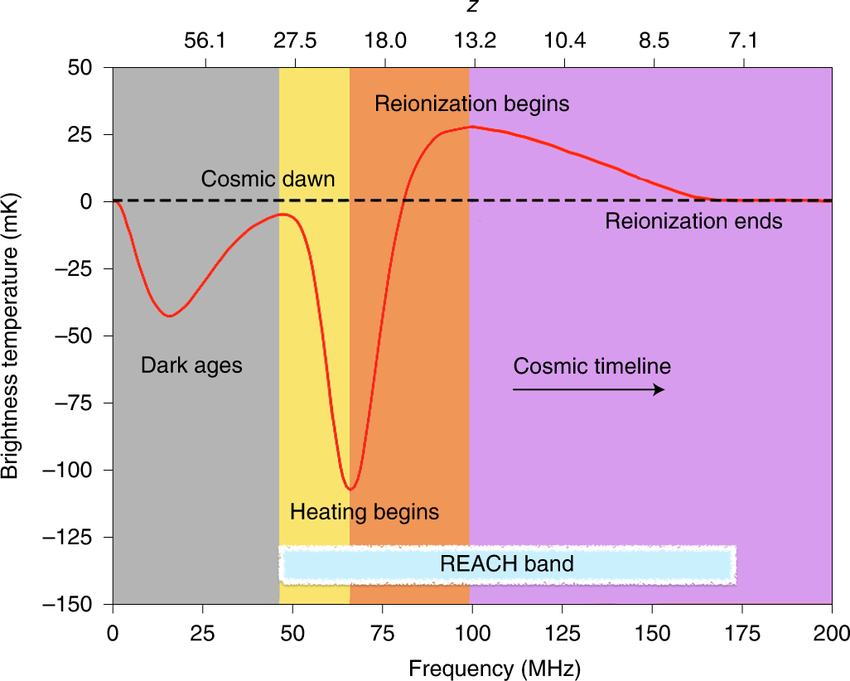
\includegraphics[width=0.68\textwidth]{images/21cm.png}
    \vspace{0.3cm}
    
    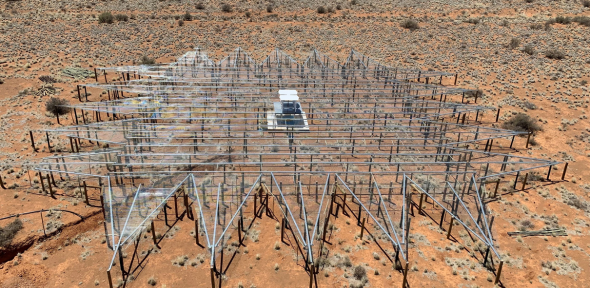
\includegraphics[width=0.85\textwidth]{images/reach.png}
    \column{0.5\textwidth}
    \centering
    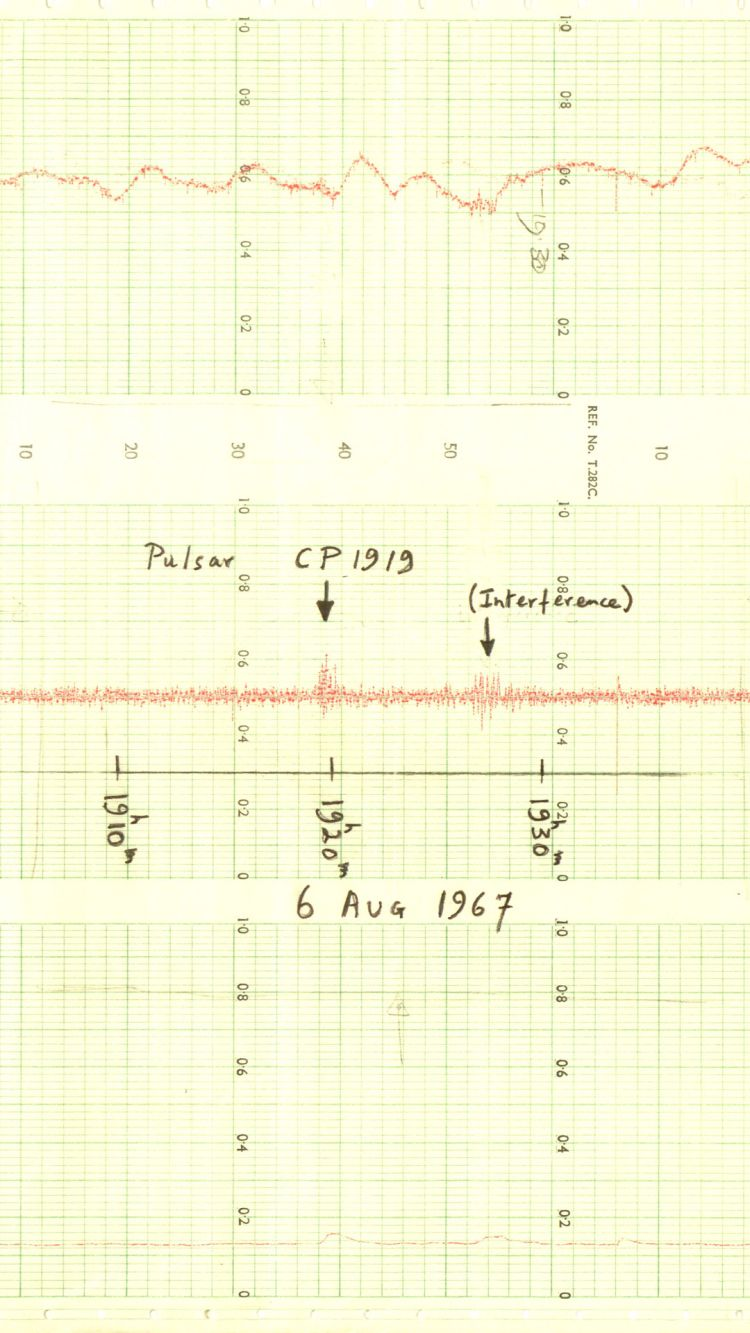
\includegraphics[width=0.55\textwidth]{images/pulsar.jpeg}
  \end{columns}
\end{frame}

\begin{frame}{Thanks for listening!}
  \vfill
  \begin{center}
    
\includegraphics[width=0.5\textwidth]{images/qr.png}
  \end{center}
  \vfill
\end{frame}

\end{document}
